
\documentclass[8pt]{article}

\usepackage[utf8]{inputenc}

\usepackage{amsmath, bm}
\usepackage{graphicx}
\usepackage{amssymb}
\usepackage{float}
\usepackage{caption}
\usepackage{subcaption}
% set font size to 11pt

% set margin
\usepackage[margin=0.5in]{geometry}

\setlength{\parskip}{\baselineskip}%
\setlength{\parindent}{0pt}%
\setlength{\voffset}{-0.75in}
\setlength{\headsep}{5pt}

\begin{document}

% insert pdf cover page here

\title{Lab report: 3F1 Flight Control}
\author{lwp26}
\date{October 2023}
\maketitle

\begin{abstract}
    \centering
    This report investigates the flight control systems of 
\end{abstract}

\newpage

\section{Introduction}

Modern control systems

\section{Manual Aircraft Control}

\subsection{Simplified Aircraft Model}

A simplified model for aircraft dynamics is given by the following equation:

\[
 \ddot{y}(t) + M\dot{y}(t) = Nx(t)
\]

Where the coefficient $M$ represents the aerodynamic damping and coefficient $N$ represents aerodynamic effectiveness of elevators.
The transfer function of this system is given by:

\begin{equation}
    G_1(s) = \frac{N}{s(s + M)}
\end{equation}

\subsection{Manual control response to impulse disturbance}

The model for manual control by a pilot is taken as a pure time delay $D$ and a gain $k$ and so for an input response $x(t)$ the output is given as $kx(t-D)$. This has a transfer function in the laplace domain as seen below.

\begin{equation}
    K(s) = ke^{-sD}
\end{equation}

\newpage

\begin{figure}[H]
    \centering
    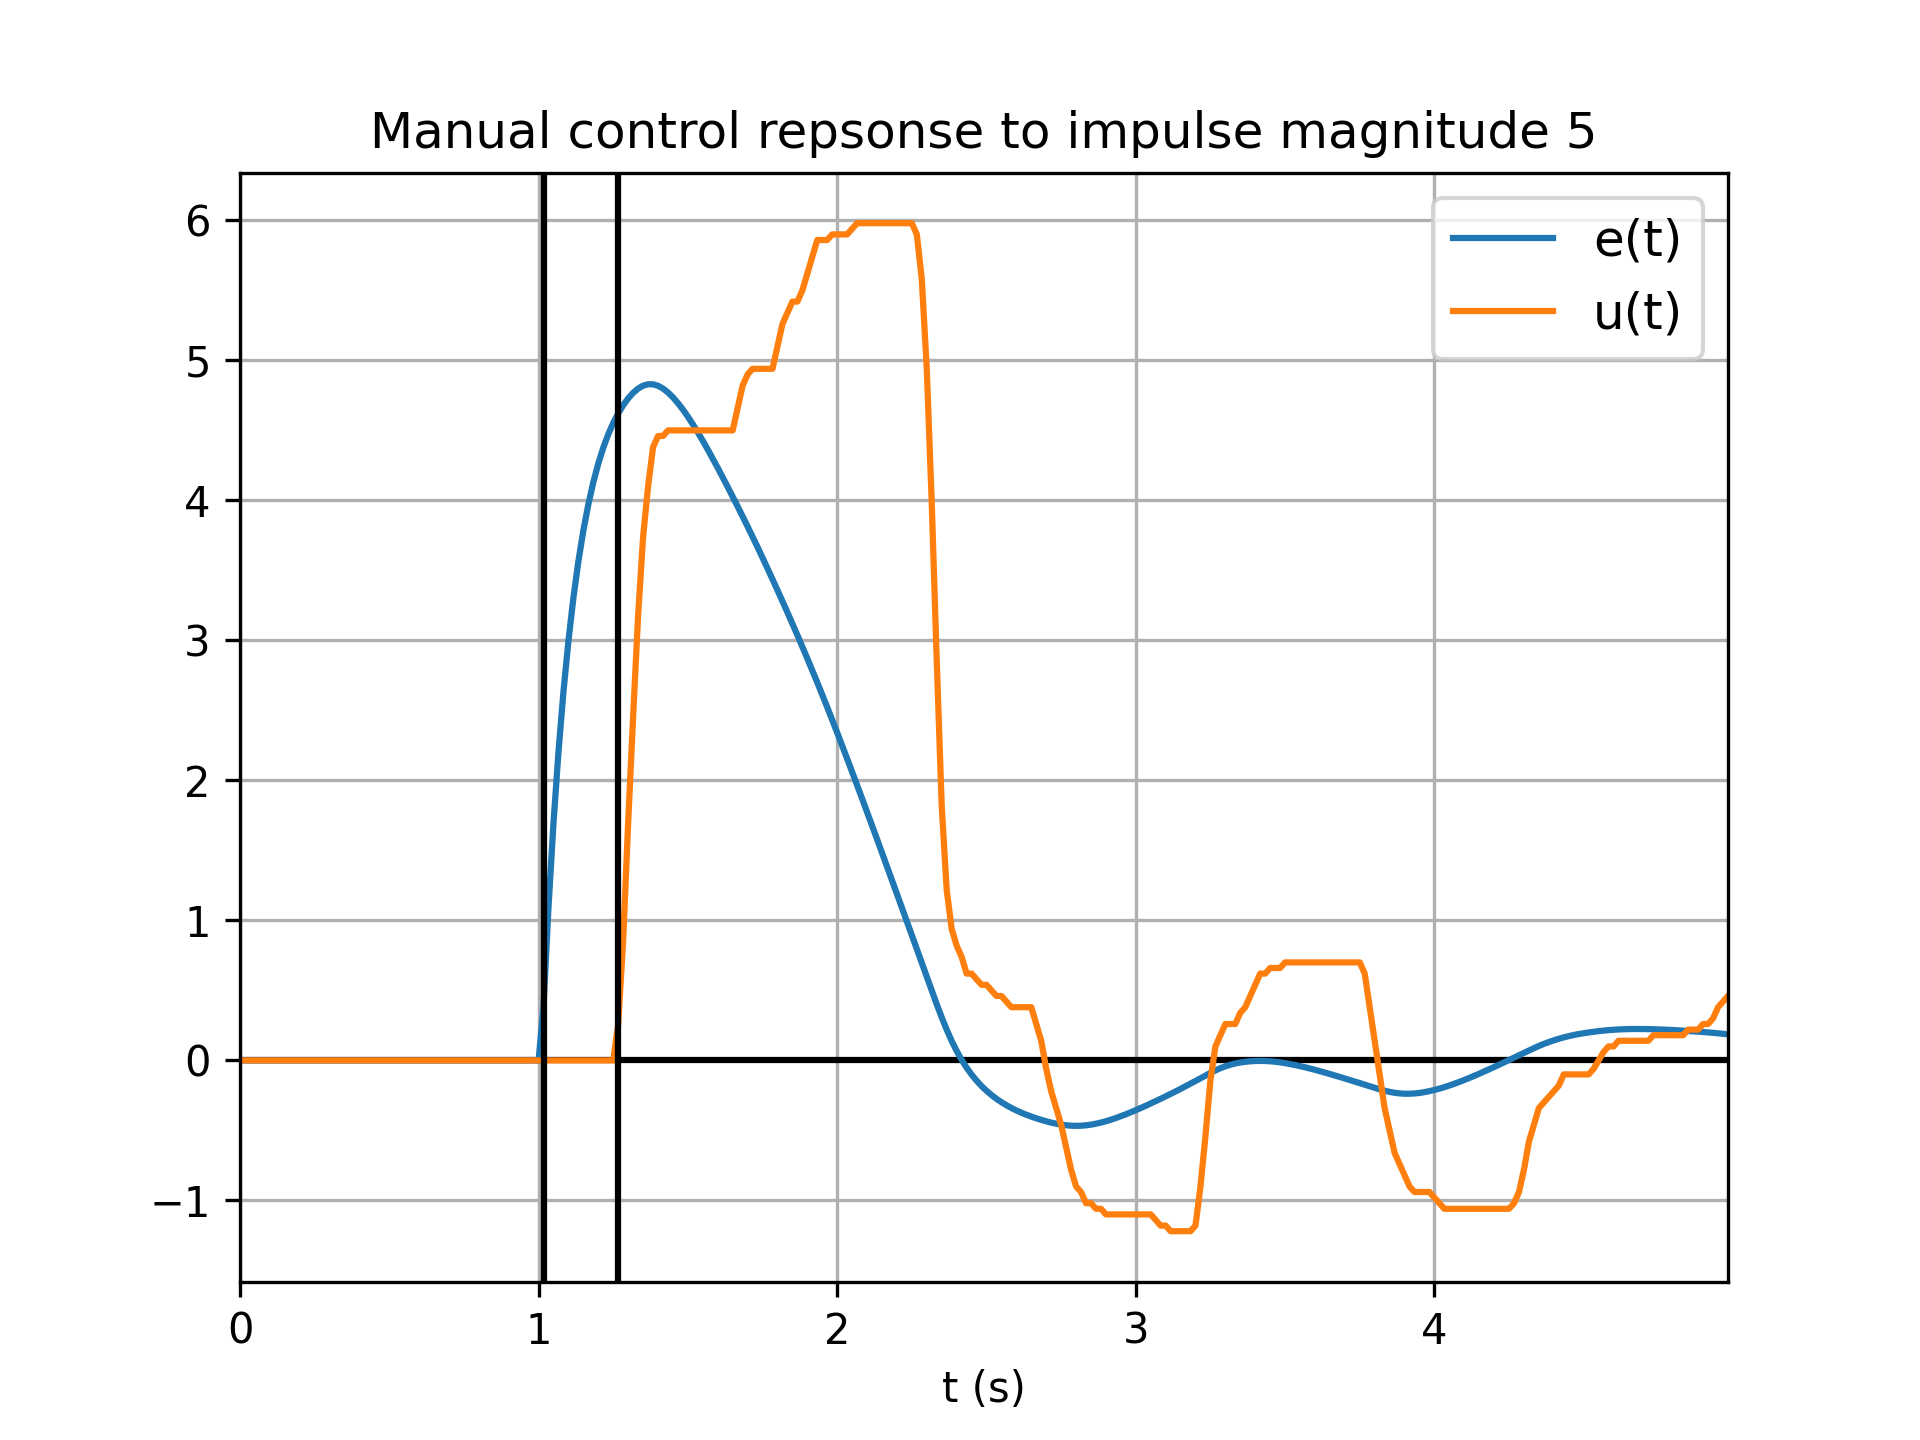
\includegraphics[width=0.6\textwidth]{figures/FIGURE_1.png}
    \caption{Manual control response graph to input disturbance to determine pilot model values of gain, $k$ and delay $D$}
    \label{fig:figure1}
\end{figure}

From Figure \ref{fig:figure1}, the gain is determined by the ratio of peak output to peak input and the time delay is determined by the time difference between the peaks of the input and output.

\begin{figure}[H]
    \centering
    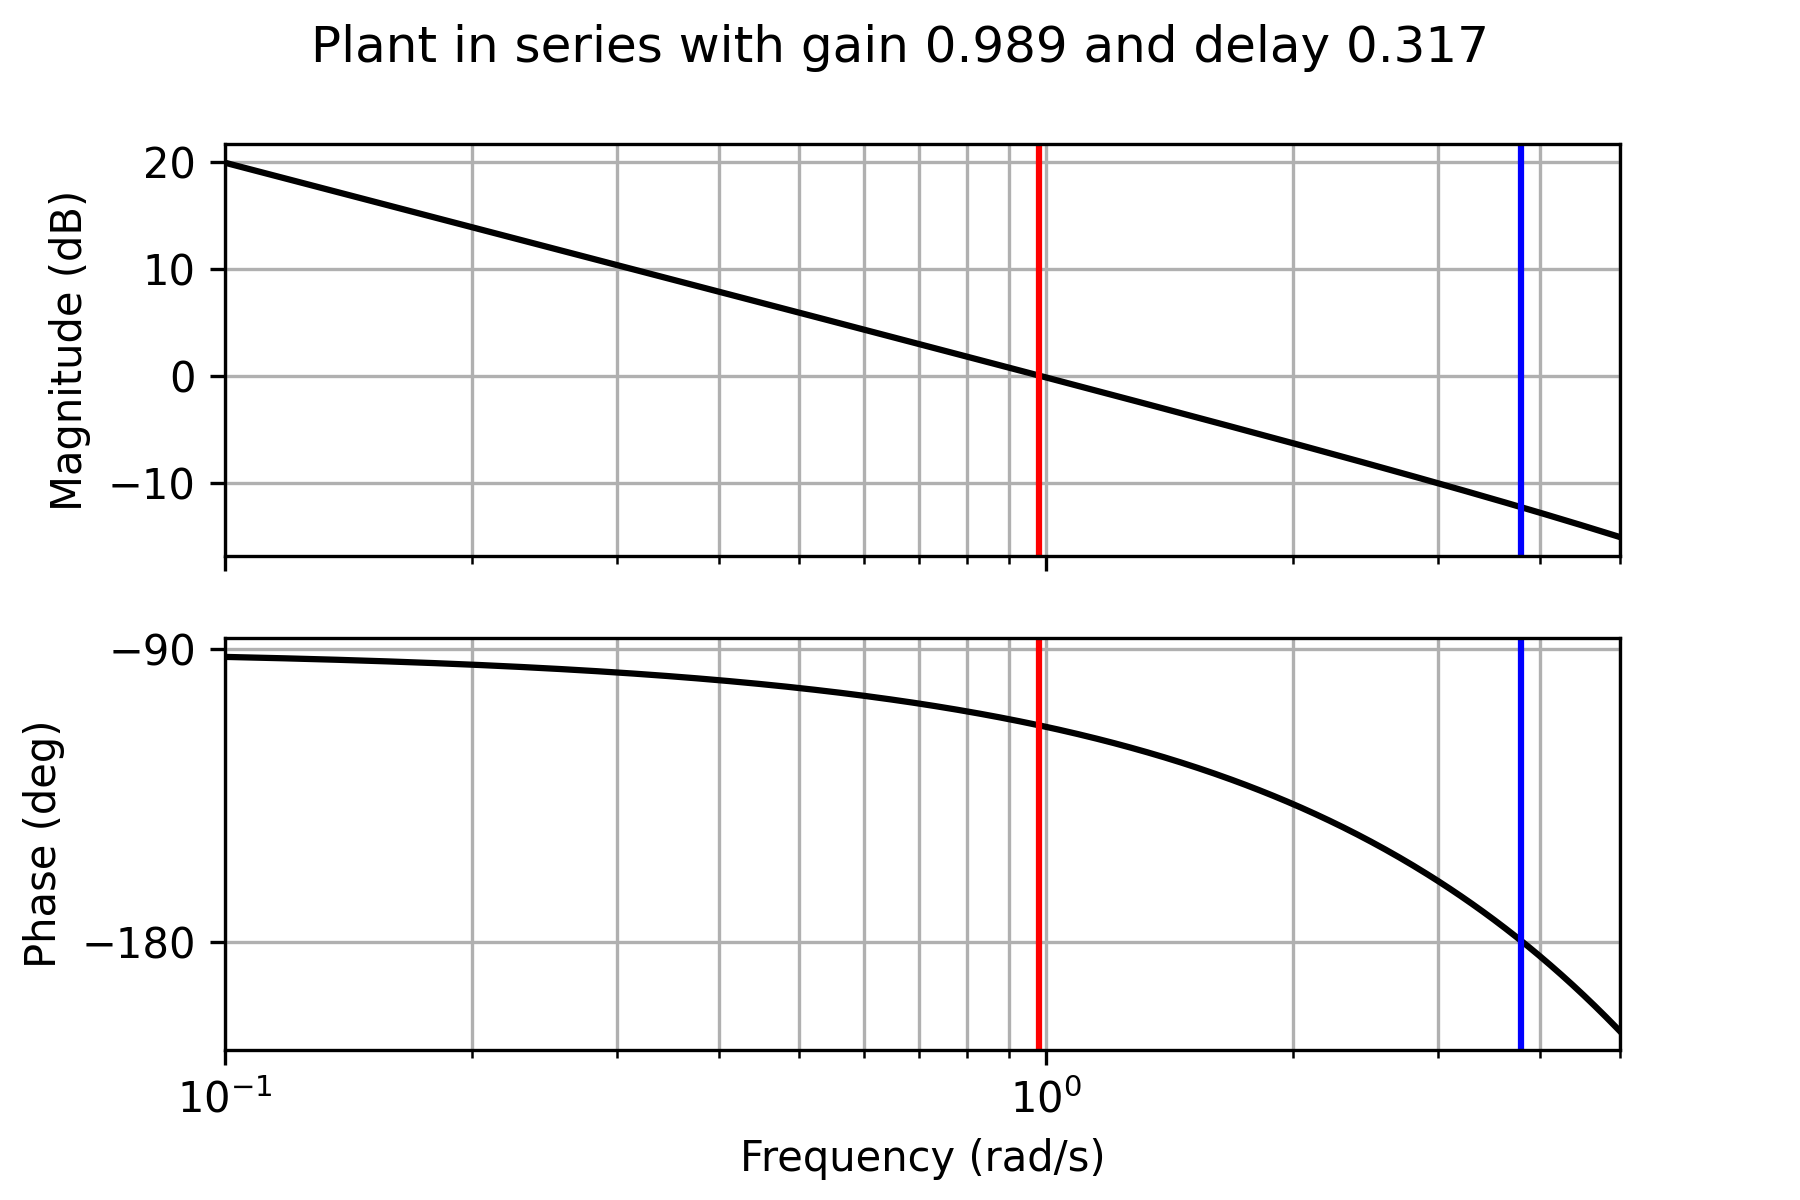
\includegraphics[width=0.6\textwidth]{figures/FIGURE_2.png}
    \caption{Bode plot of open loop manual control model, $K(j\omega)G(j\omega)$}
    \label{fig:figure2}
\end{figure}

From Figure \ref{fig:figure2}, the gain margin is found using the gain on at the blue line at at -180 degrees phase. This was found to be $4.10$.
The phase margin is found using the phase difference with -180 on the red line where the gain is 0dB. This was found to be $66.6$ degrees. Both of these points correspond to where the nyquist plot encircles the $-1$ point.

If the gain of 0.989 were to remain unchanged, from the frequency of $\omega = 0.980$ rad/s at the phase margin of $66.6$ degrees, or $1.16$ rad, the additional time delay before unstability be found to be $1.19$ s.

\begin{figure}[H]
    \centering
    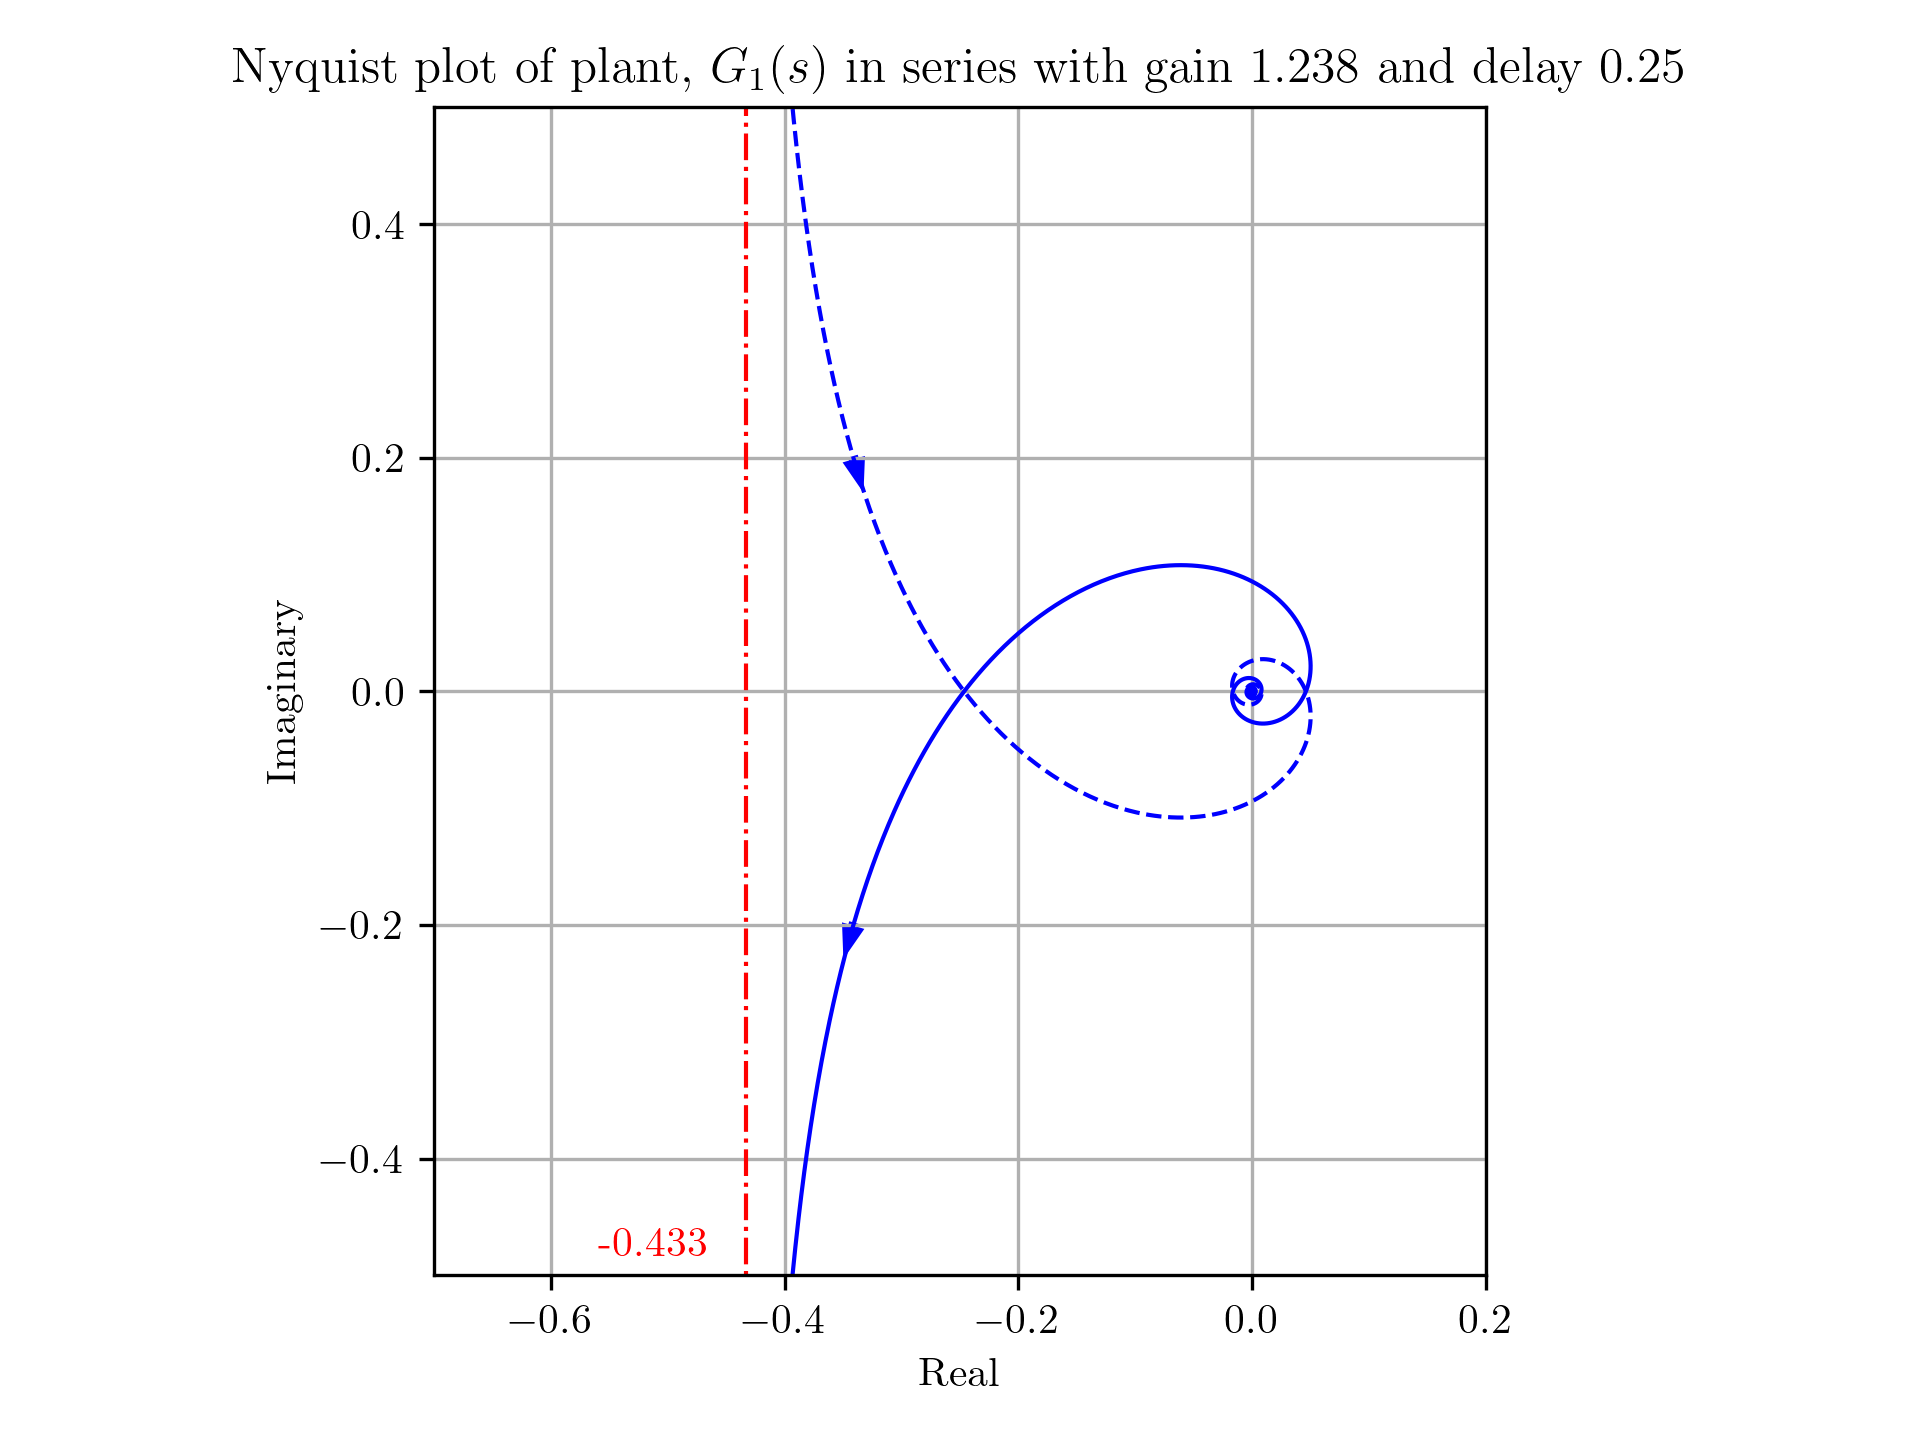
\includegraphics[width=0.8\textwidth]{figures/nyquist1.png}
    \caption{Nyquist plot for open loop manual control model, $K(j\omega)G(j\omega)$}
    \label{fig:nyquist1}
\end{figure}
% could do additional nyquist plots at cases of gain and phase margins.

\subsection{Manual response to step input distrubance}

\begin{figure}[H]
    \centering
    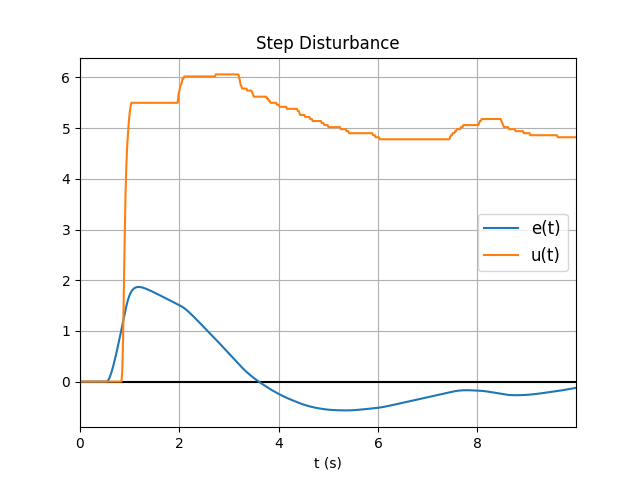
\includegraphics[width=0.8\textwidth]{figures/FIGURE_3.png}
    \caption{}
    \label{fig:figure3}
\end{figure}

In Figure \ref{fig:figure3} the manual control to the step response can be seen. It can be seen that integral action is used here, as to minimise the error signal $e(t)$ to 0, the input signal $u(t)$ must equal a constant, which can only be achieved by an intergator.
The original model for the controller without the intregral term would have a large error.

The response is still delayed, $D$ to the error signal, but now with an intergator term, so we would expect the new controller to take the form of:

\begin{equation}
    K(s) = e^{-sD}\left( k + \frac{1}{sT_i}\right)
\end{equation}

\section{Pilot Induced Oscillation}

Considering an aircraft of poorly designed control system with the transfer function.

\begin{equation}
    G_1(s) = \frac{c}{(Ts+1)^3}
\end{equation}

Where parameters are chosen as functions of pilot controller model: $T=4D/\pi$ and $c=\sqrt{8}/k$
An impulse response of $5kD$ is shown below in Figure \ref{fig:figure4}.

\begin{figure}[H]
    \centering
    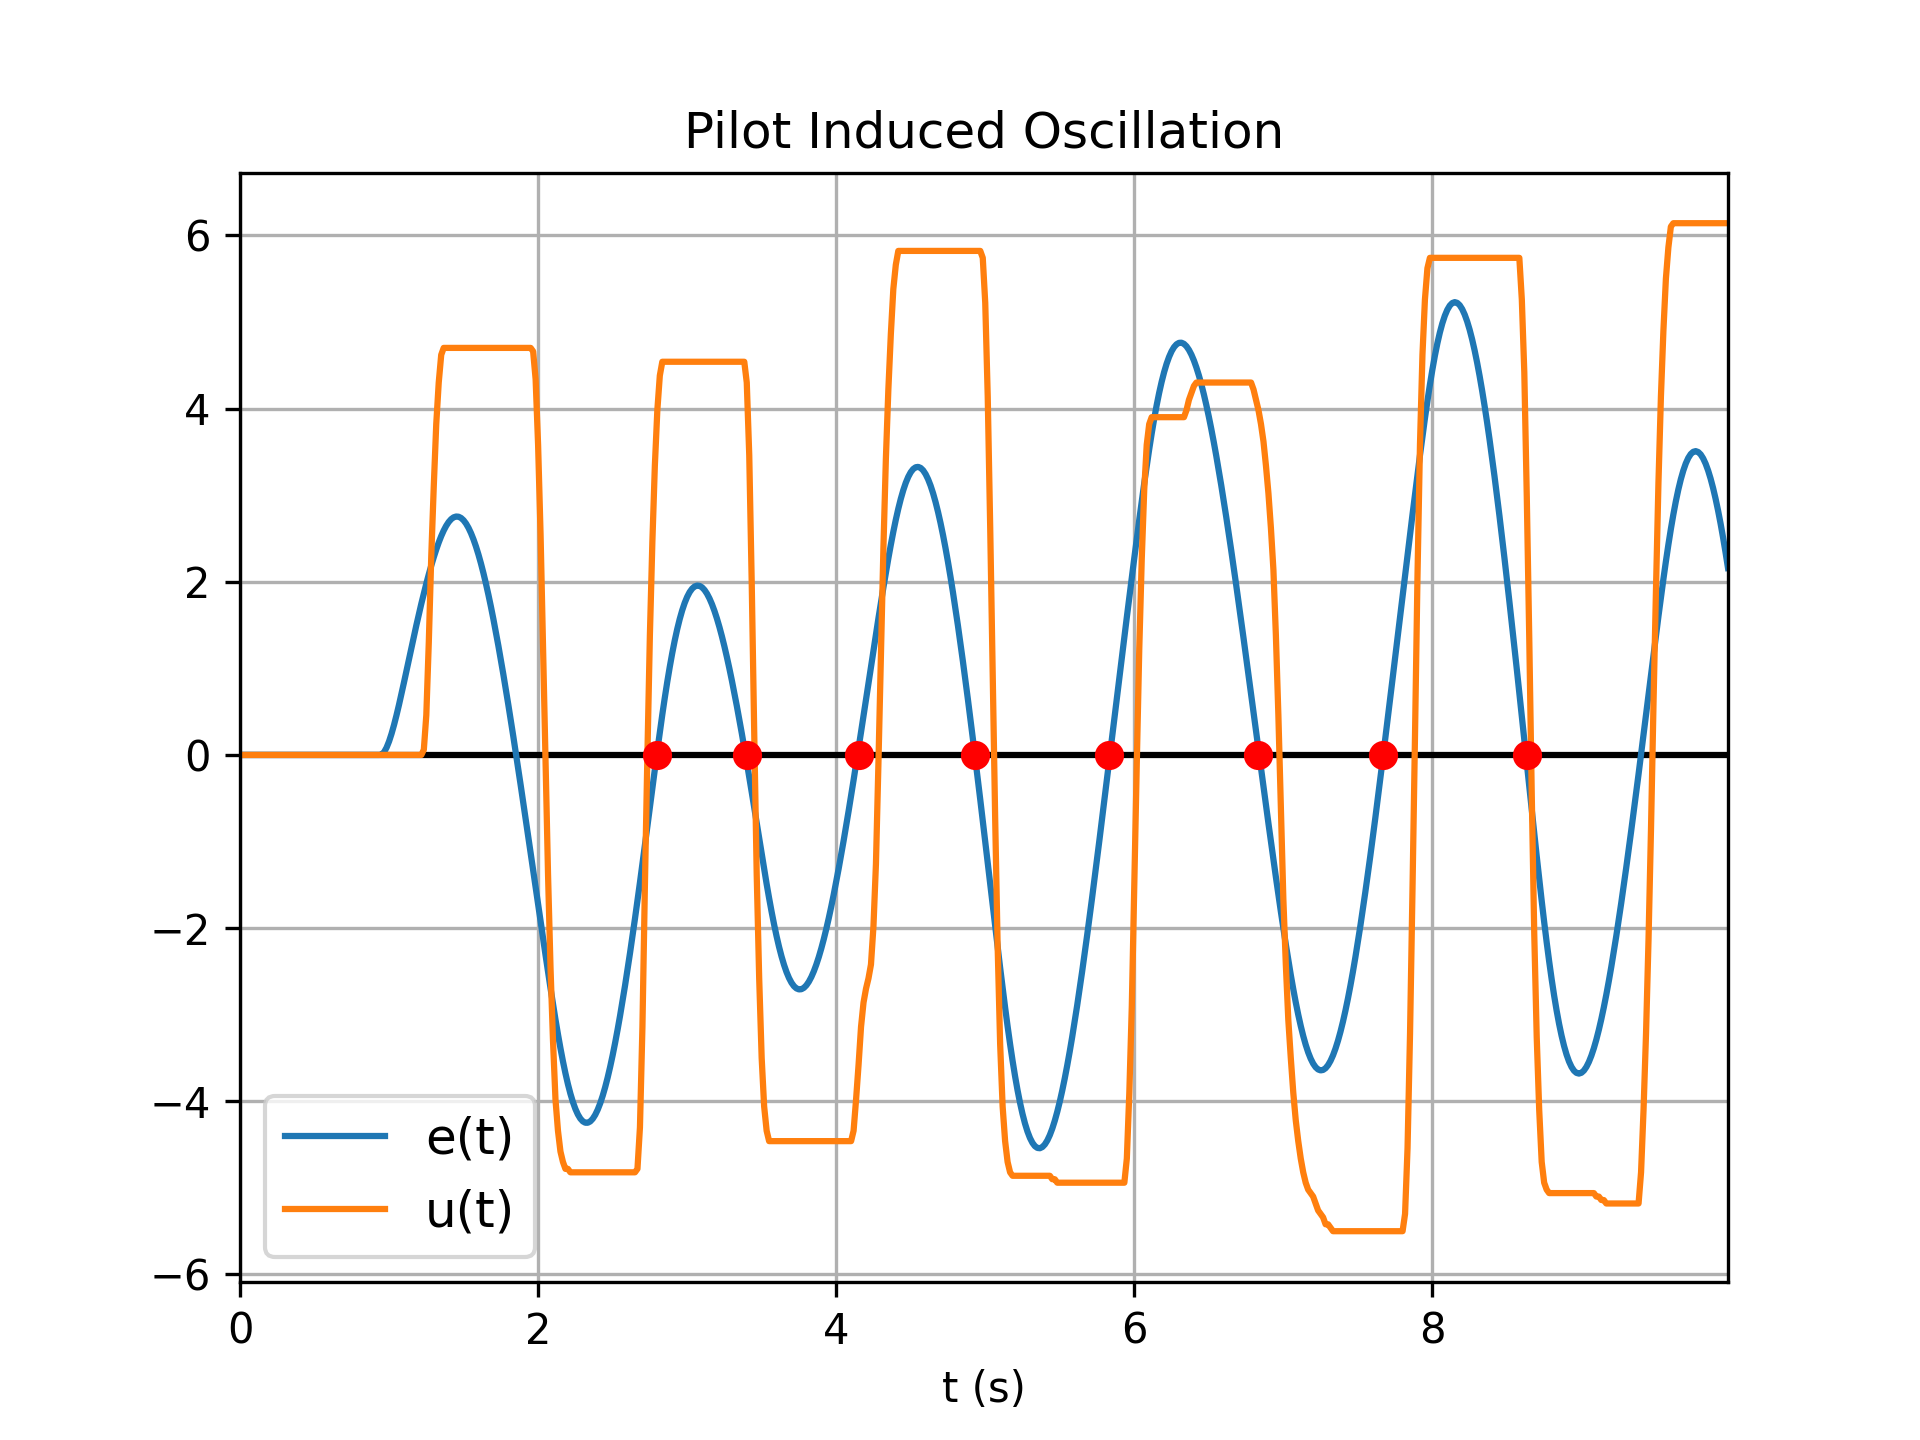
\includegraphics[width=0.8\textwidth]{figures/FIGURE_4.png}
    \caption{Manual control response to impulse of weight $5kD$}
    \label{fig:figure4}
\end{figure}

3. Explain the oscillation of the feedback loop. How does your observed period of oscillation compare to the theoretical prediction of the feedback loop?

This shows a highly oscillatory response triggered by an impulse disturbance.
The average period of which is $1.672$ s, as calculated from where the error signal intersects the x axis shown by the red points.
This gives an angular frequency of $3.758$ rad/s.

The response for the modelled pilot controller, with same gain and delay as before is shown below in Figure \ref{fig:figure5}.

\begin{figure}[H]
    \centering
    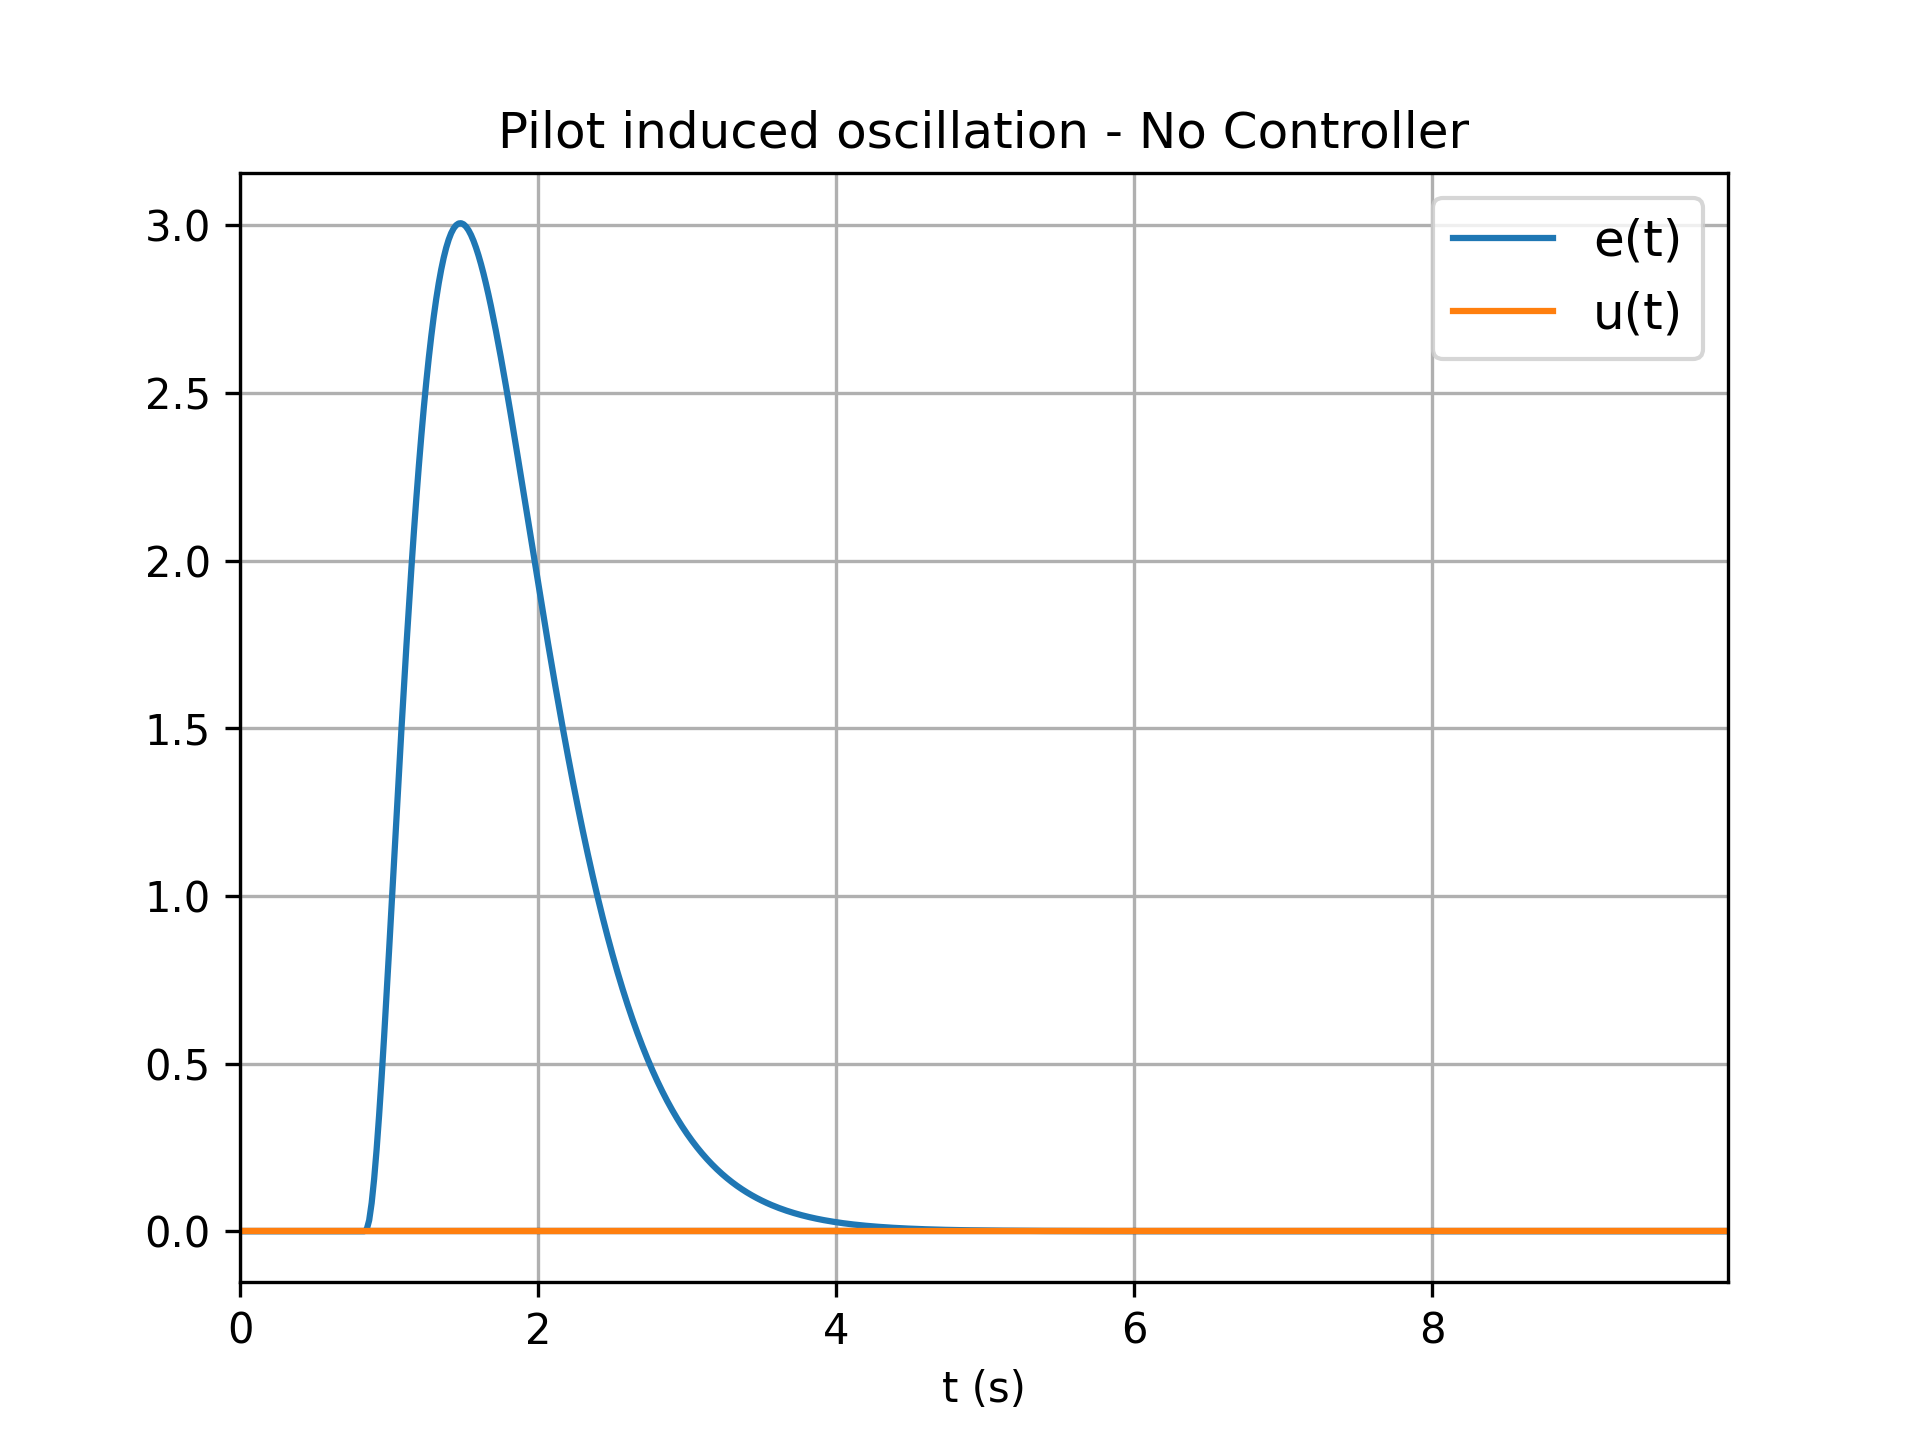
\includegraphics[width=0.8\textwidth]{figures/FIGURE_5.png}
    \caption{No controller response to impulse of weight $5kD$ }
    \label{fig:figure5}
\end{figure}

In Figure \ref{fig:figure5} without a controller, shows no oscillatory response, to the same impulse disturbance.

\begin{figure}[H]
    \centering
    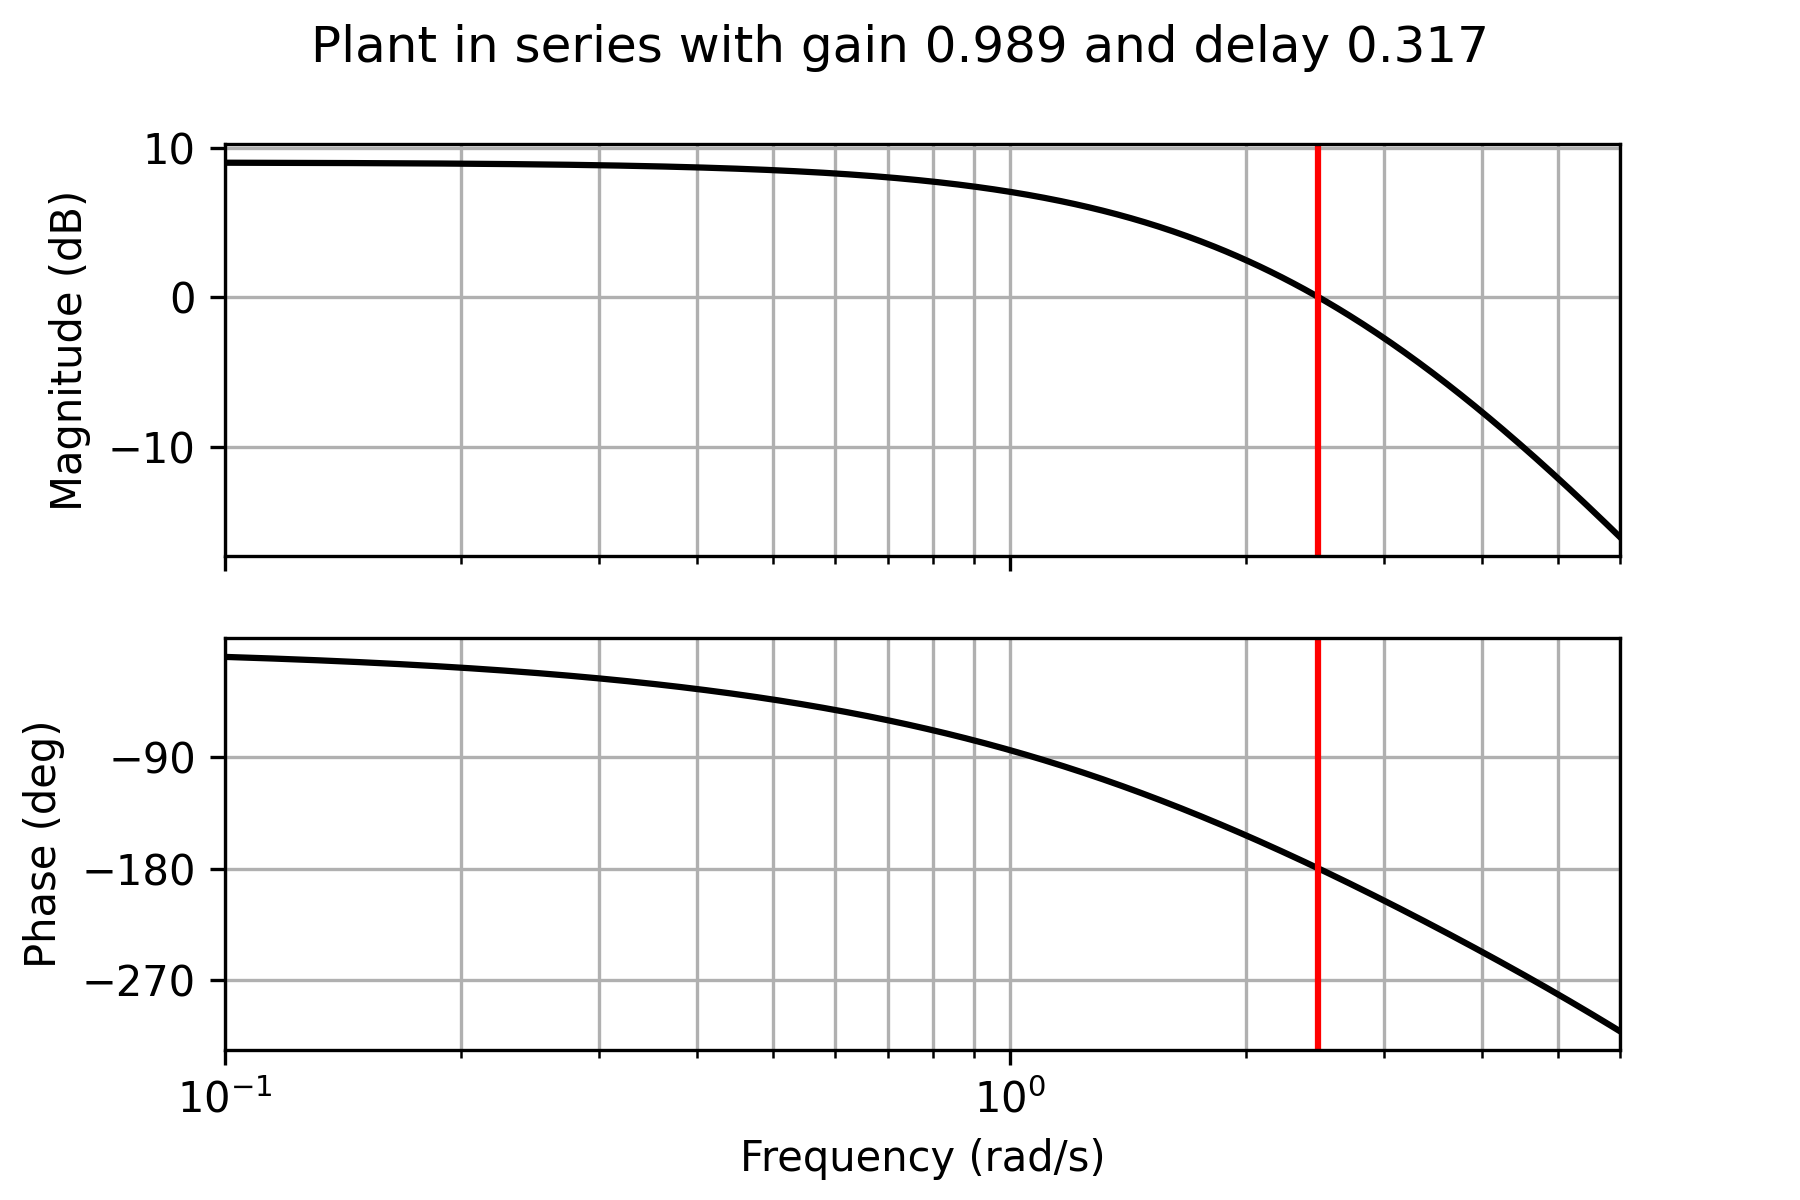
\includegraphics[width=0.8\textwidth]{figures/FIGURE_6.png}
    \caption{Bode plot of, $K(j\omega)G(j\omega)$}
    \label{fig:figure6}
\end{figure}

Figure \ref{fig:figure6} shows the bode plot of the plant, $G_2(j\omega)$, with the model pilot controller.
The gain and phase margins are found the same way as before and are found to be, 0.997 and 0.212 degrees respectively.
This shows, as the gain margin is less than 1, that the system is unstable. However, as its very close to 1, it can be considered marginally stable.

At this point of unstability, the frequency is found to be $\omega = 2.473$ rad/s, which corresponds to a theortical period of $2.540$ s.
This period of oscillation, is much larger than the period of oscillation of the real manual controller, which was $1.672$ s.

explain the oscillation of the feedback loop. How does your observed period of oscillation compare to the theoretical prediction of the feedback loop?
Can you give a rough guideline to the control system designer to make PIO less likely?

\section{Sinusoidal Disturbances}

For this section, the control system of a F4E fighter jet is analysed during sinusoidal distrubances.
The fighter jet has various operating points, which are shown below.

Point 1 Altitude 5000ft. Mach 0.5
Point 2 Altitude 5000ft. Mach 0.85
Point 3 Altitude 35000ft. Mach 0.9
Point 4 Altitude 35000ft. Mach 1.5

Only operating point 4 is analysed in this report.

\begin{figure}[H]
    \centering
    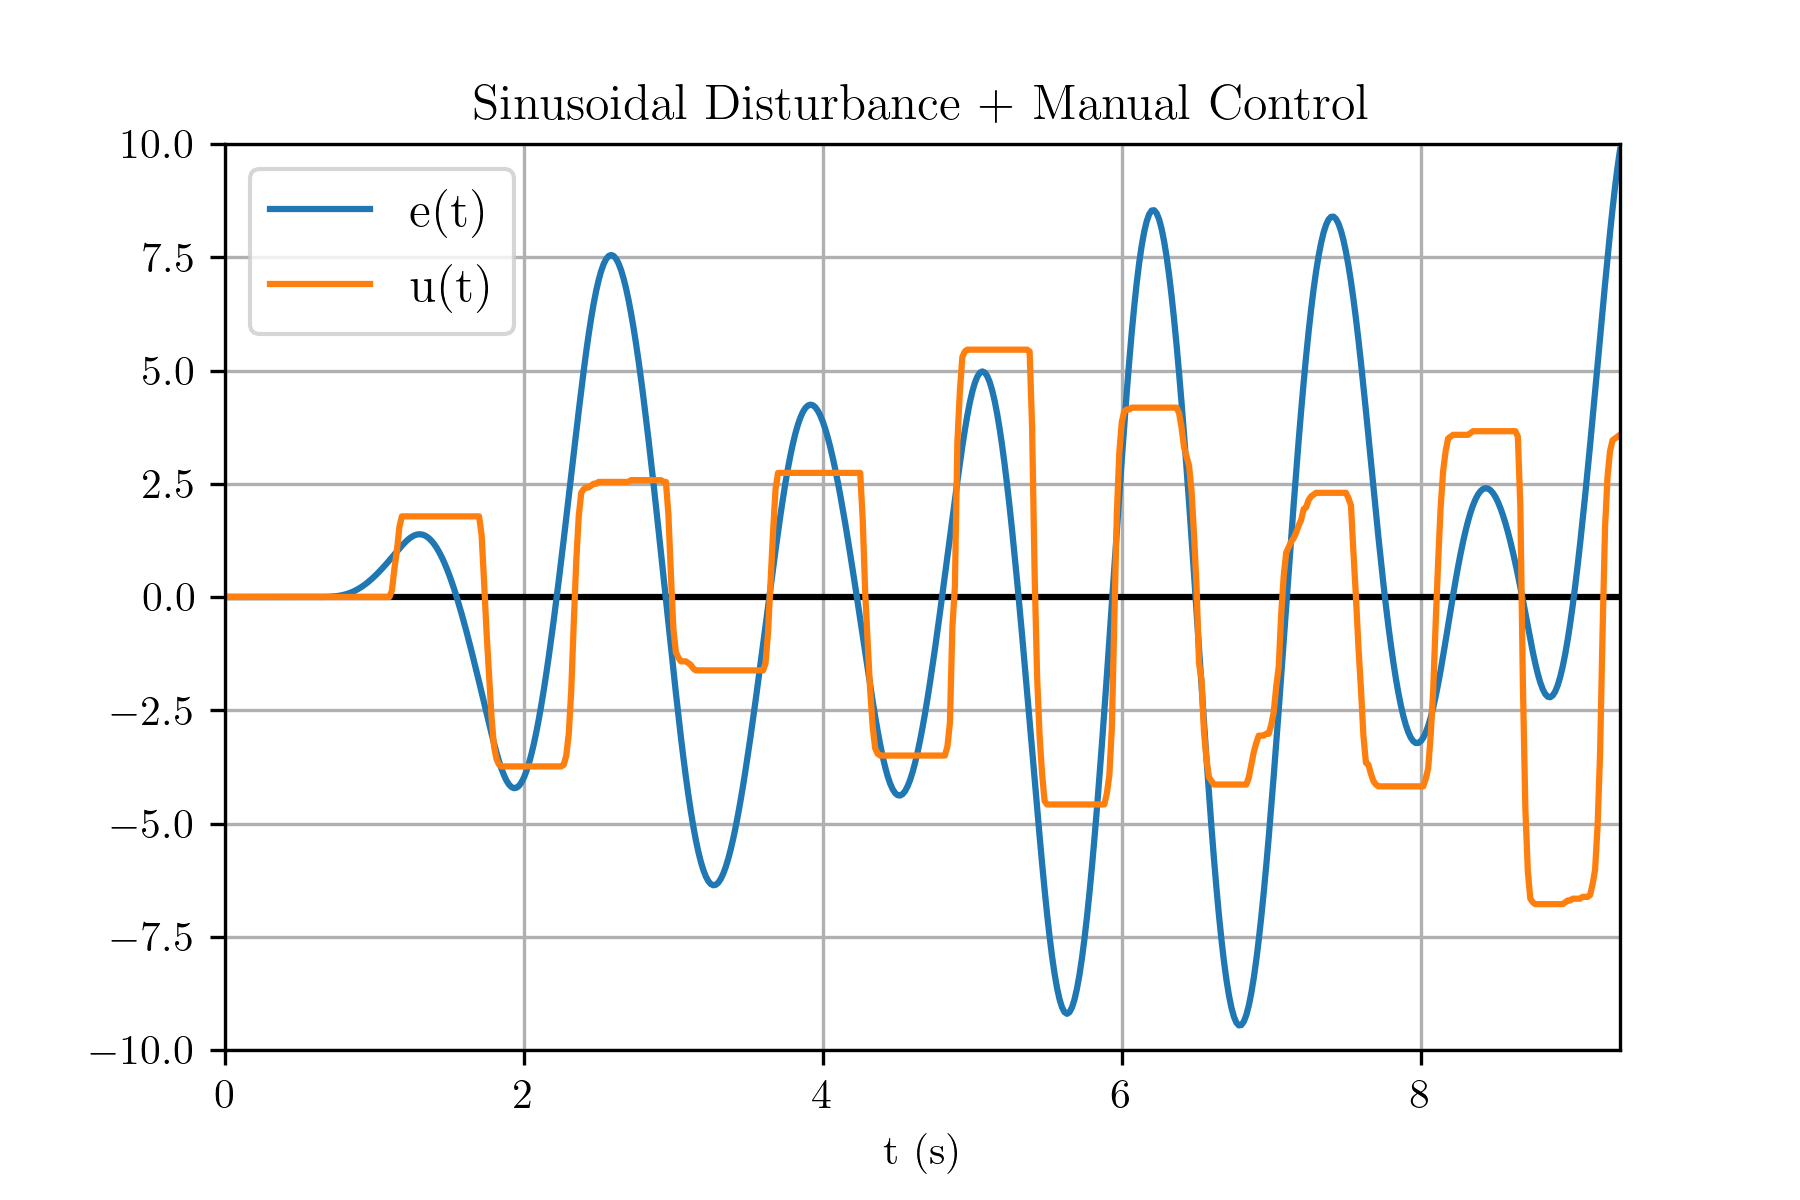
\includegraphics[width=0.8\textwidth]{figures/FIGURE_7.png}
    \caption{Manual control input response with disturbance at $0.66$ Hz}
    \label{fig:figure7}
\end{figure}

\newpage

\begin{figure}[H]
    \centering
    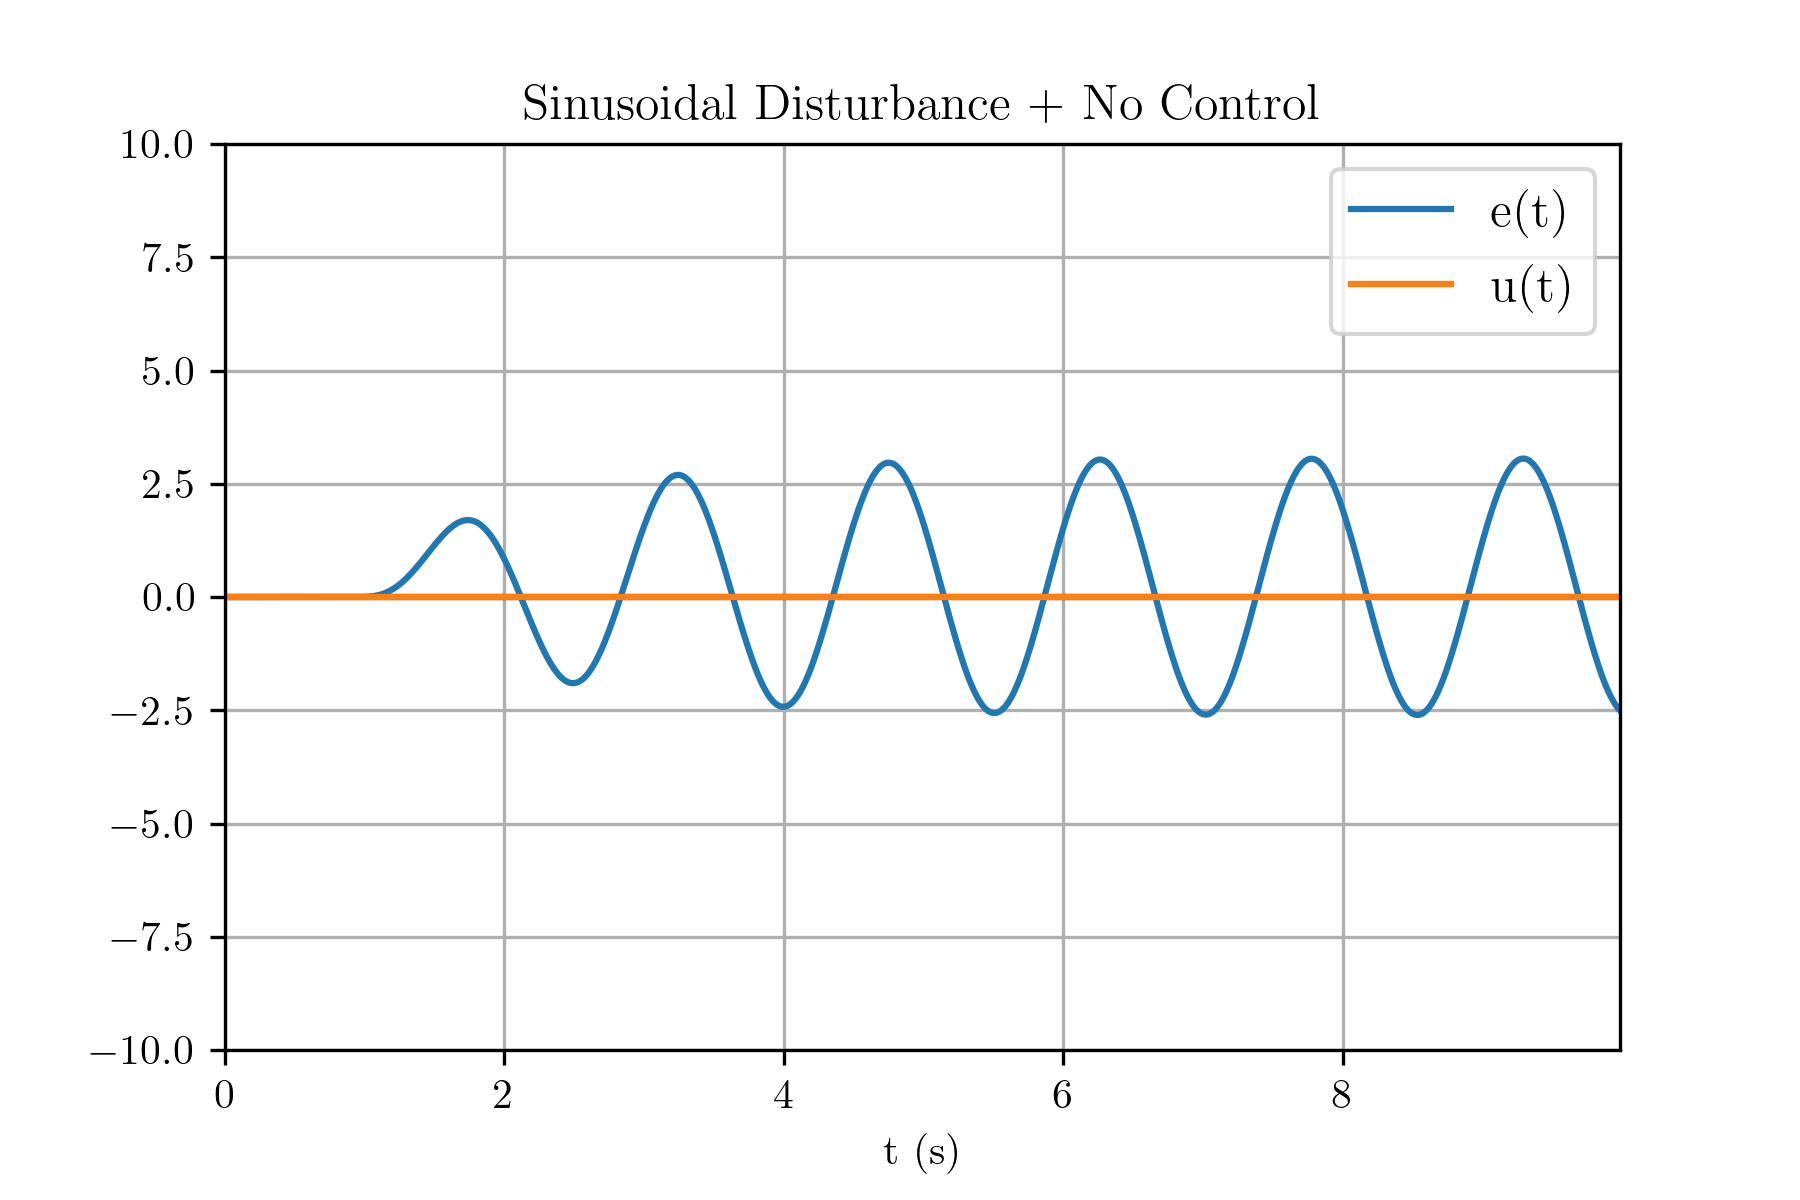
\includegraphics[width=0.8\textwidth]{figures/FIGURE_8.png}
    \caption{No control input response to disturbance at $0.66$ Hz}
    \label{fig:figure8}
\end{figure}

\begin{figure}[H]
    \centering
    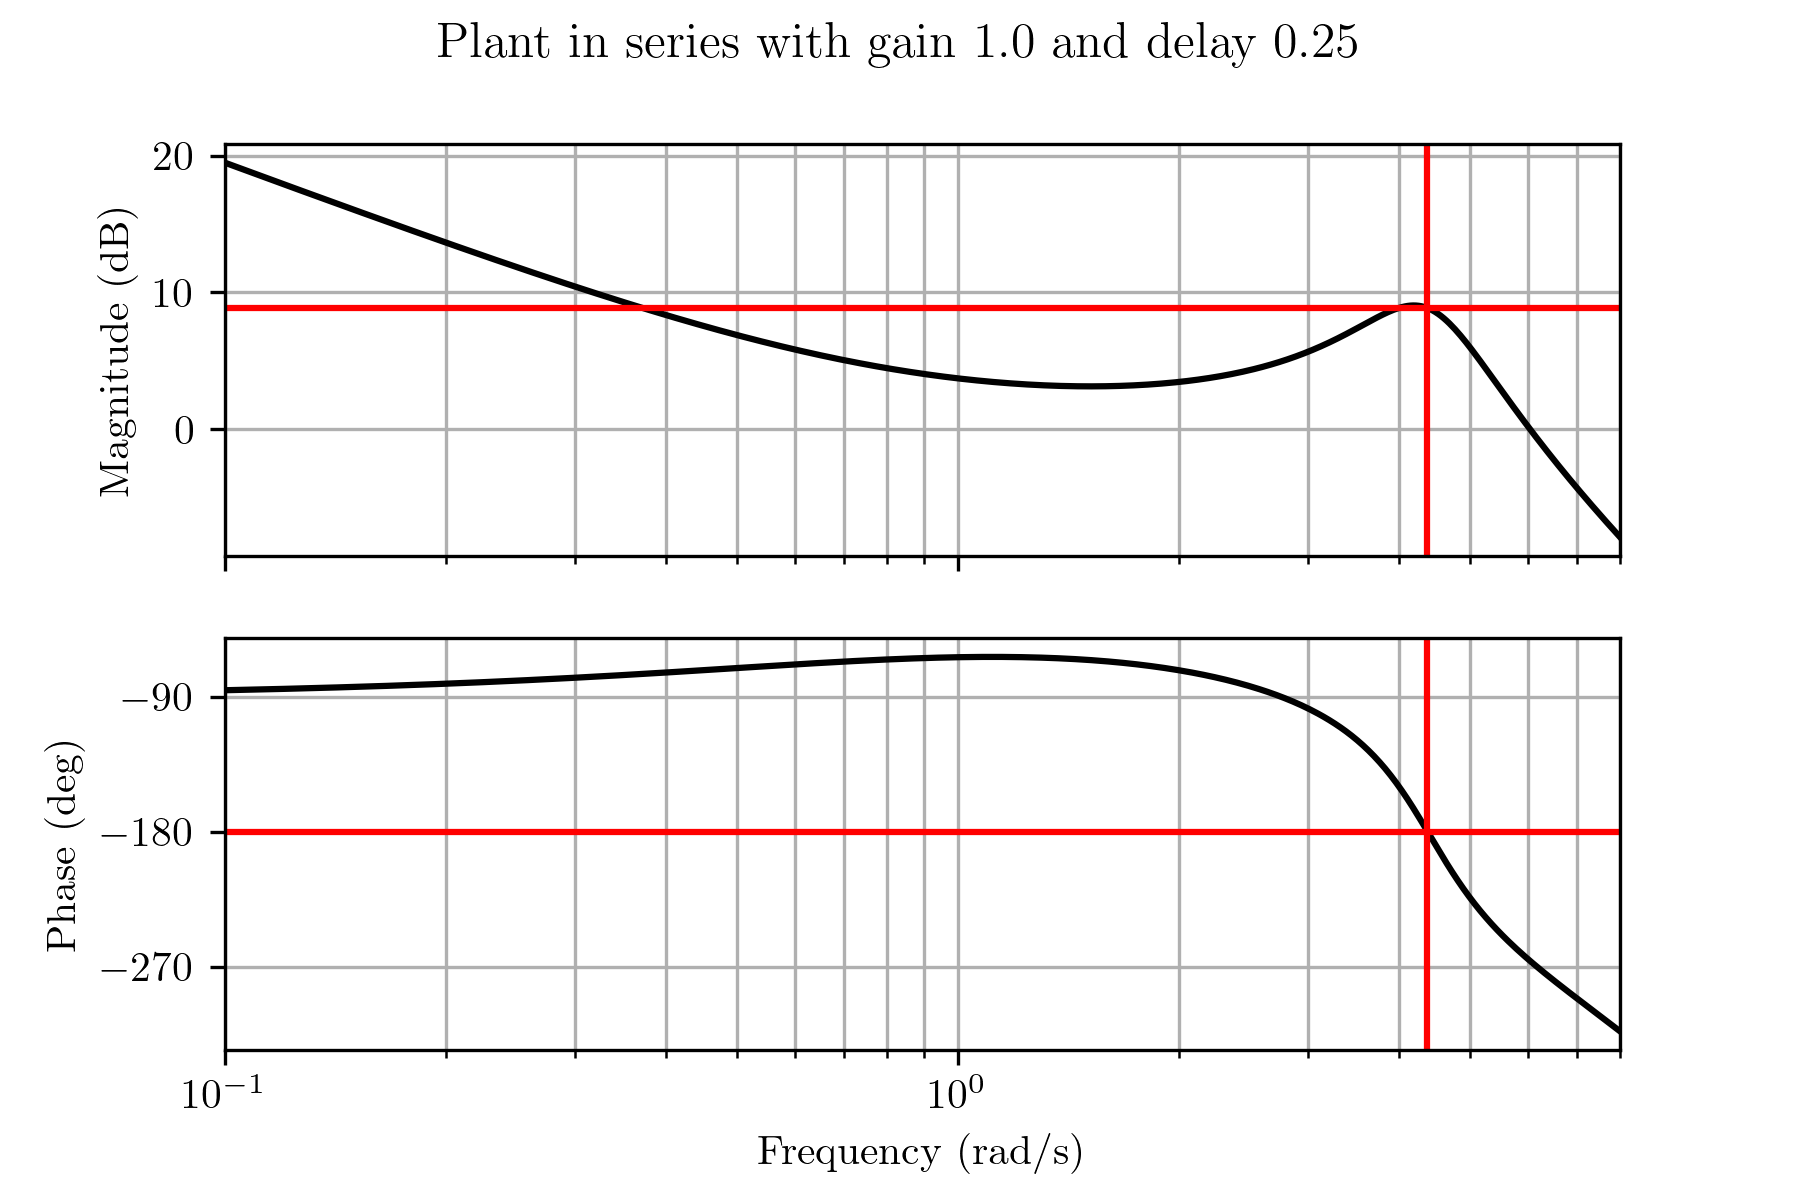
\includegraphics[width=0.8\textwidth]{figures/FIGURE_9.png}
    \caption{Bode plot for F4E fighter jet with controller of gain $1.0$ and time delay $0.317$ s}
    \label{fig:figure9}
\end{figure}

The bode plot shown in Figure \ref{fig:figure9} shows a point of resonance at $\omega = 4.147$ rad/s or $0.66$ Hz.

The gain margin for this system is 0.3527, which is the maximum gain for which the system is stable.
This shows that stability could be achieved at small ampltidues

\newpage

\begin{figure}[H]
    \centering
    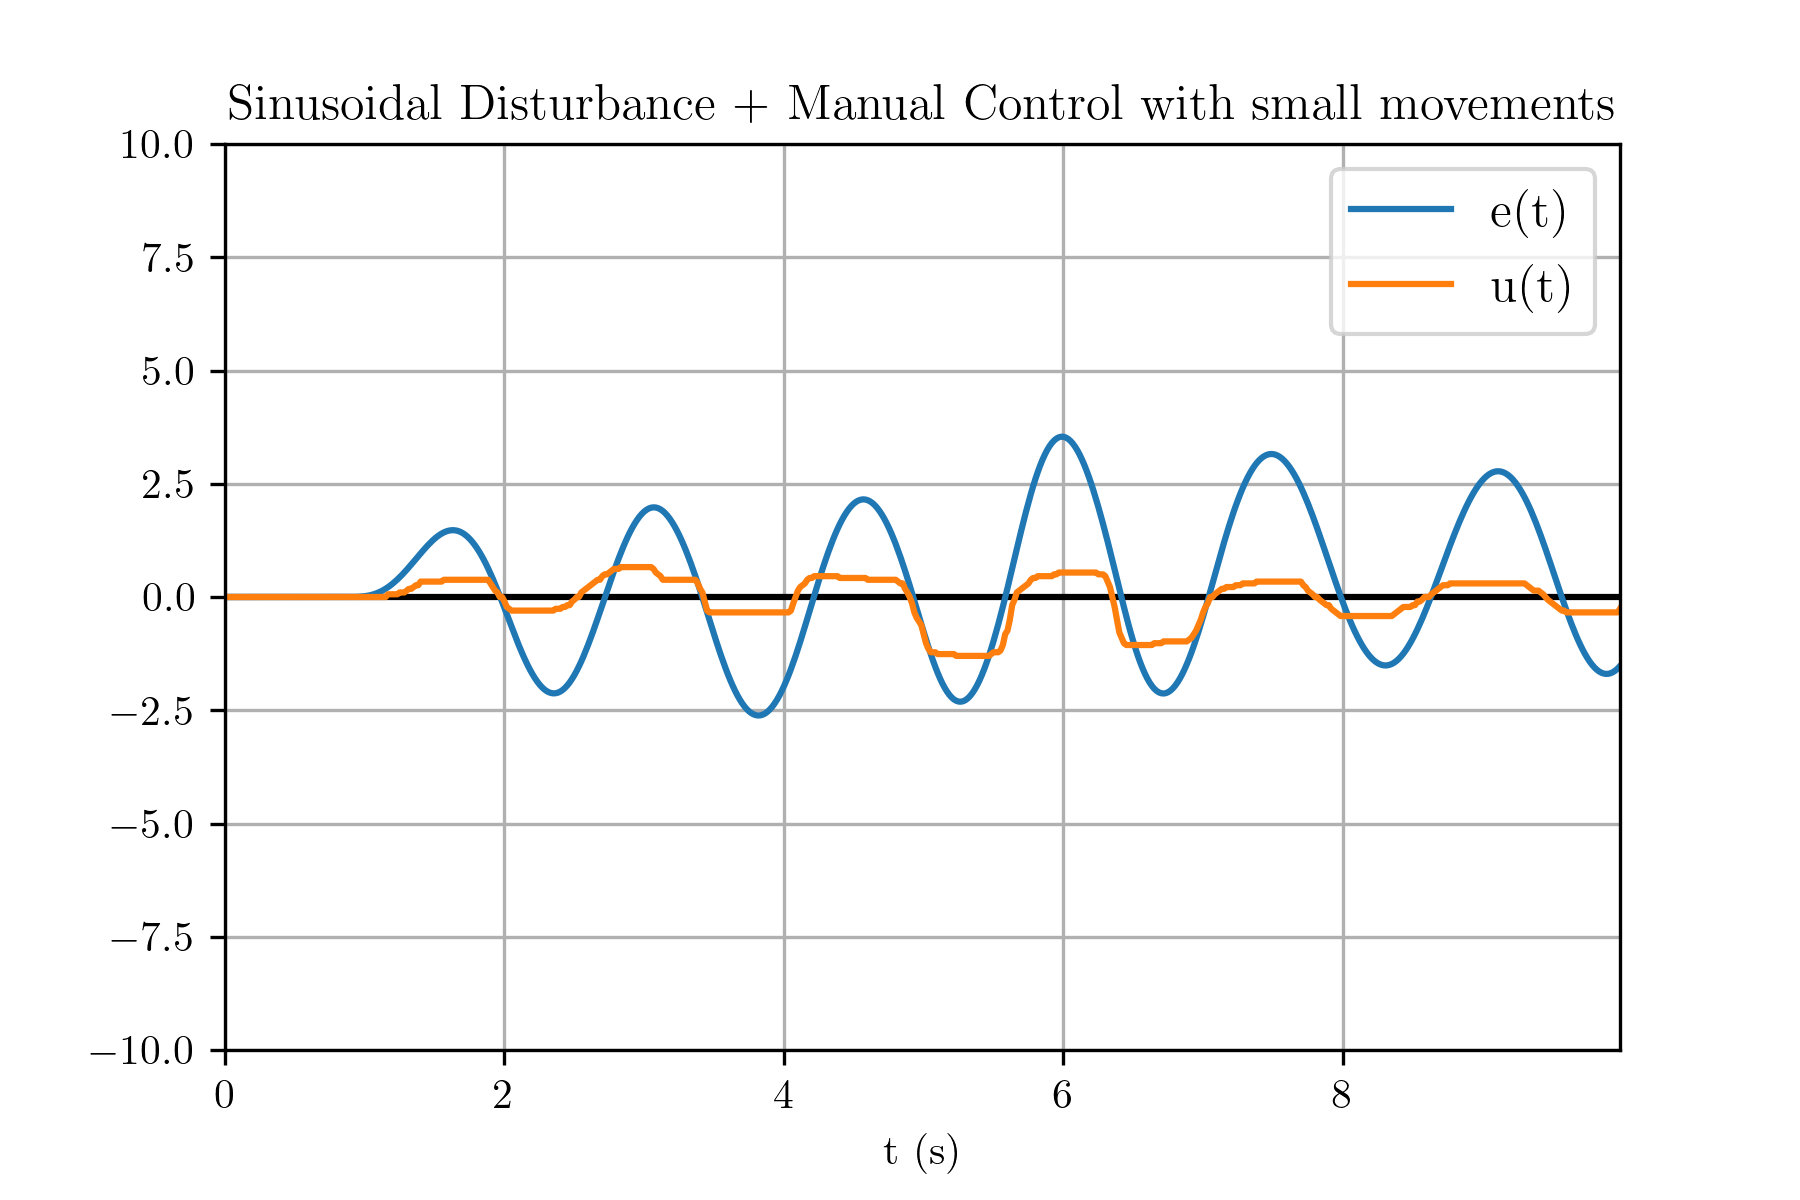
\includegraphics[width=0.8\textwidth]{figures/FIGURE_10.png}
    \caption{Figure 10}
    \label{fig:figure10}
\end{figure}

Figure \ref{fig:figure10} shows the response to small control movements. This shows better system stability than the previous manual input responses.

Was your manual control able to reduce the error compared to no input? Compare all three cases (manual control, no control, manual control with small movements).

\section{Unstable Aircraft}

\begin{equation}
    G_2(s) = \frac{2}{Ts-1}
\end{equation}

\begin{figure}[H]
    \centering
    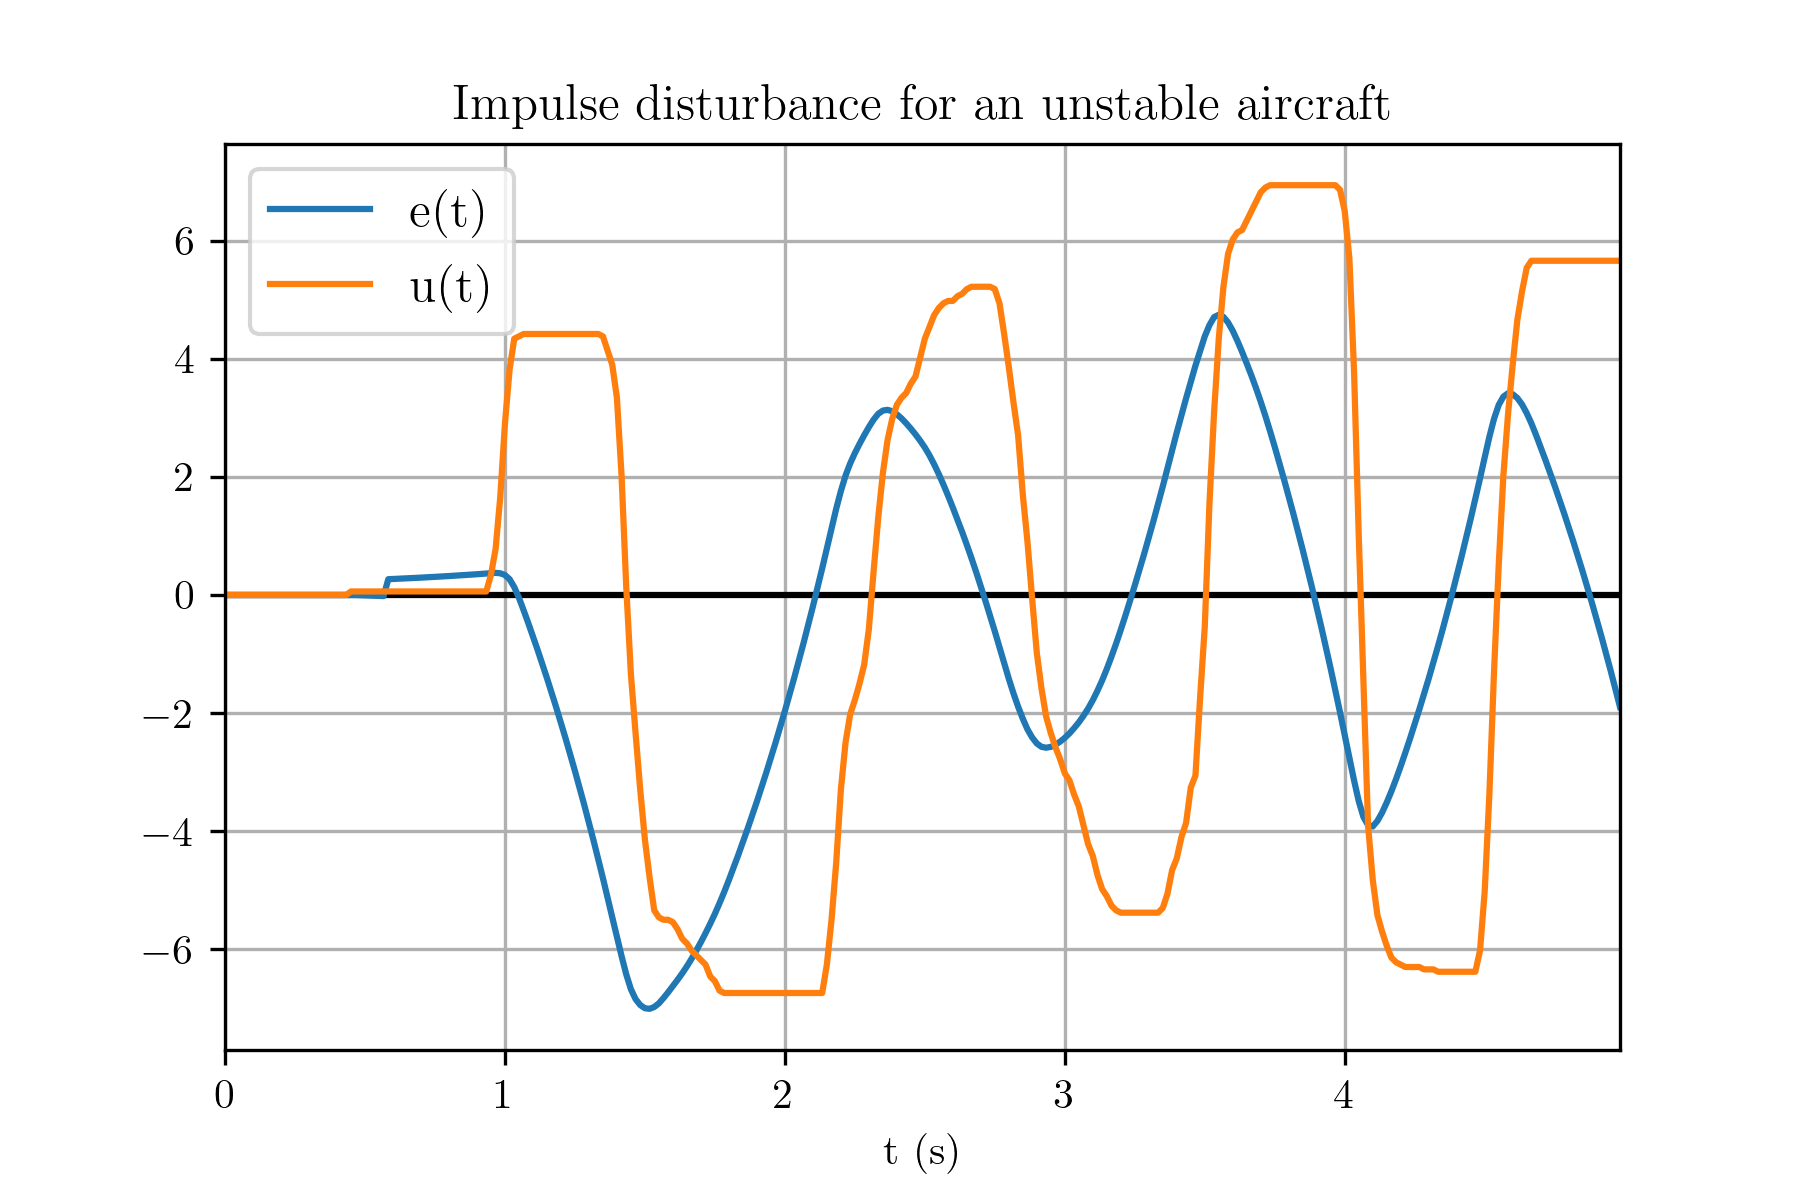
\includegraphics[width=0.8\textwidth]{figures/FIGURE_11.png}
    \caption{Manual control response to 0.1 magnitude impulse with $T=0.55$}
    \label{fig:figure11}
\end{figure}

Figure \ref{fig:figure11} shows manual control response

6. Nyquist diagram for $G_2(j\omega)$
\begin{figure}[H]
    \centering
    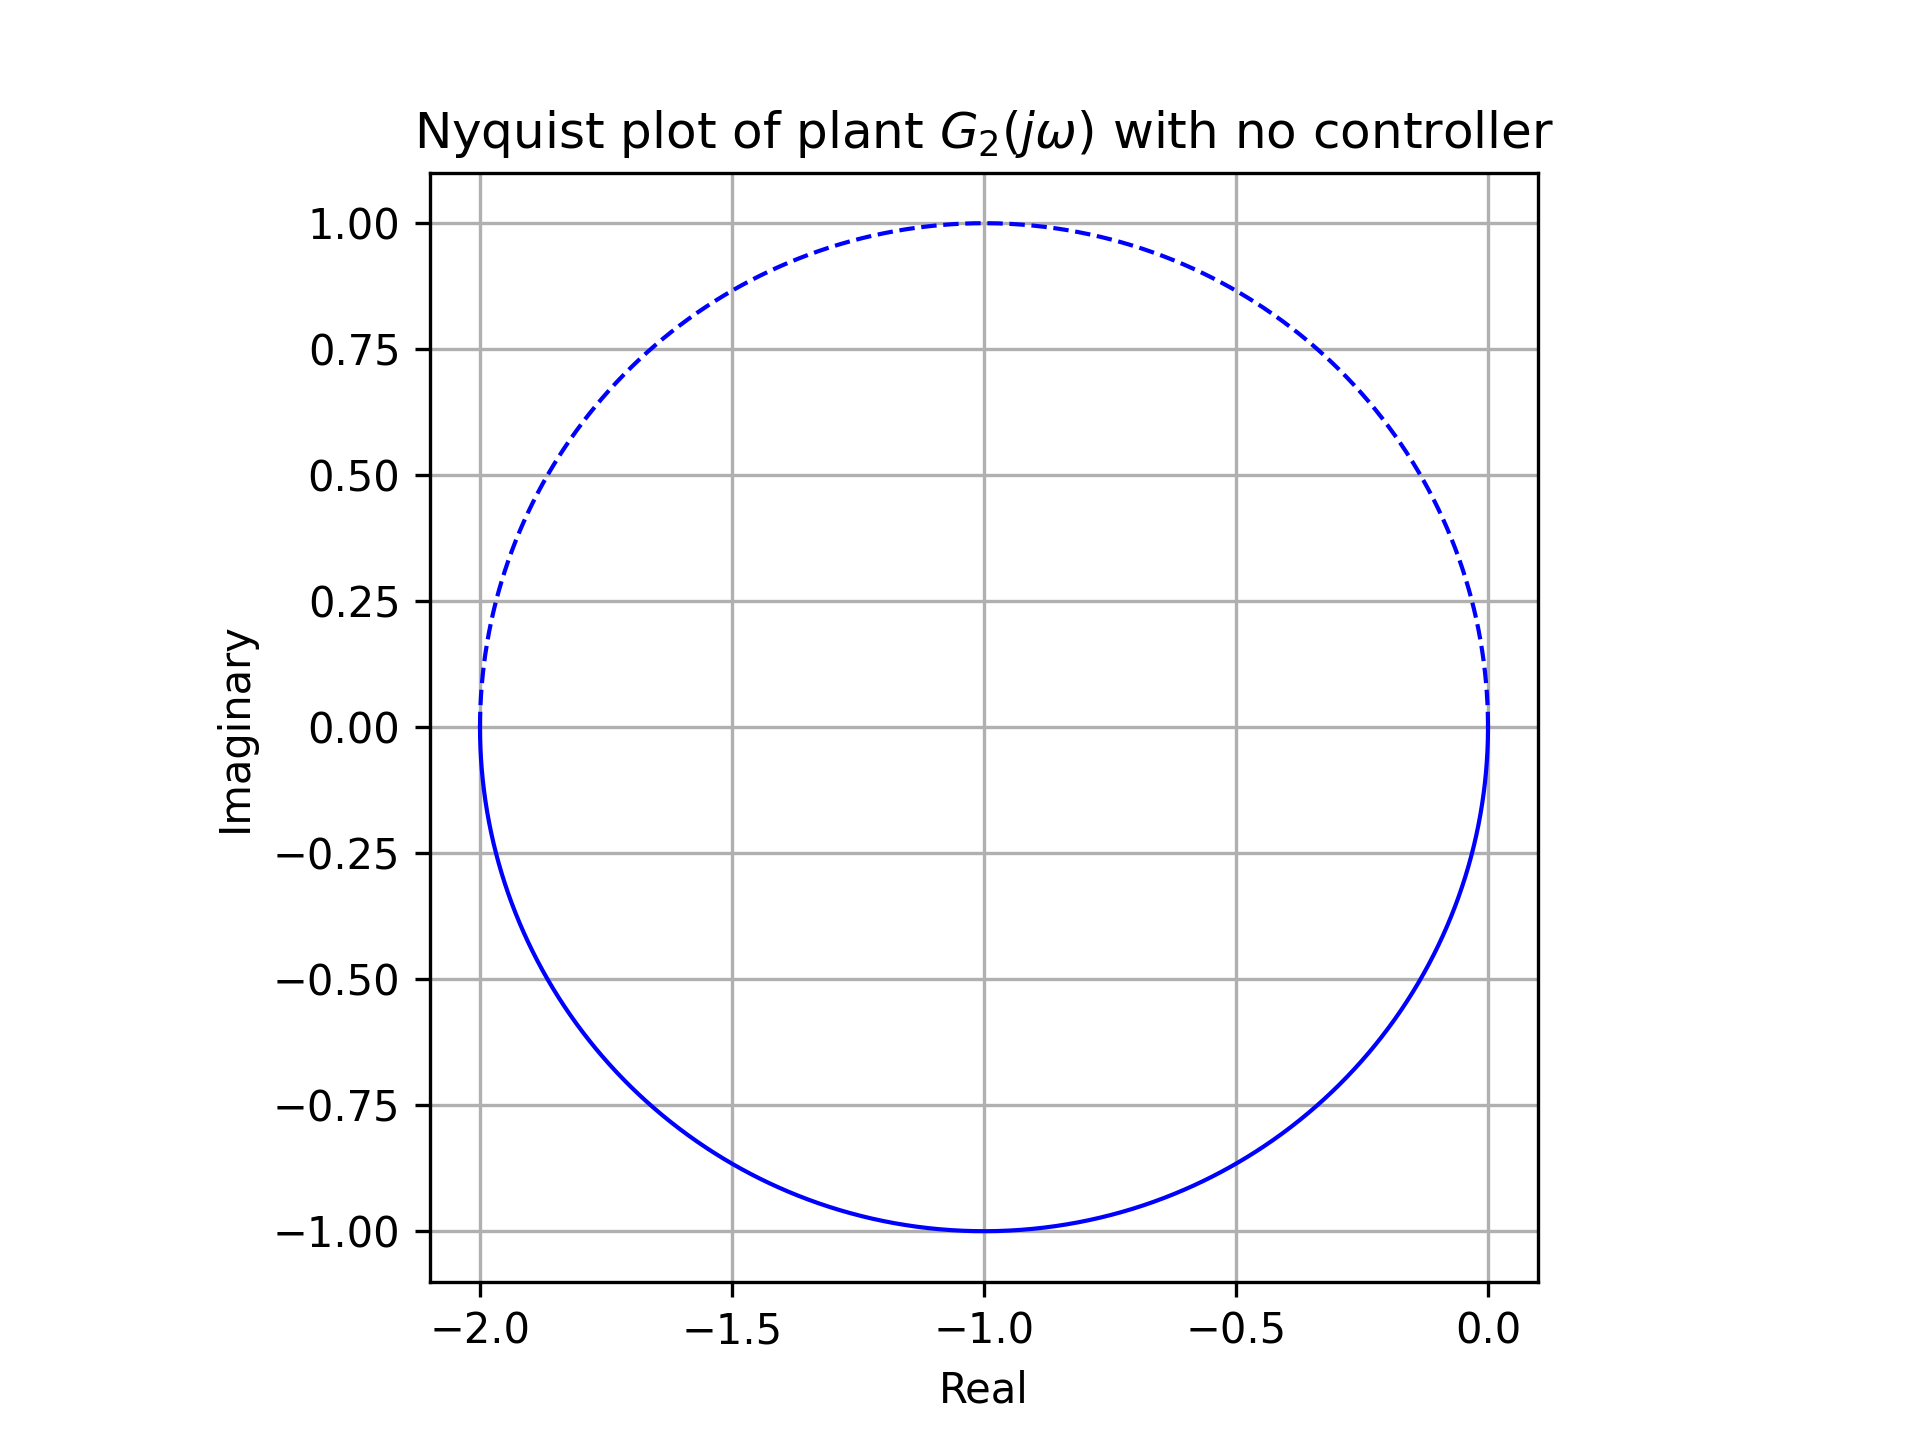
\includegraphics[width=0.8\textwidth]{figures/nyquist2.png}
    \caption{Nyquist plot of plant, $G_2(j\omega)$}
    \label{fig:nyquist2}
\end{figure}
7. Explain, using the Nyquist criterion, why the feedback system is stable with a proportional gain greater than 0.5

Explaination using nyquist criterion

8. Finally, show how the Nyquist diagram is modified if a small time delay $D$ is introduced to the system.
\begin{figure}[H]
    \centering
    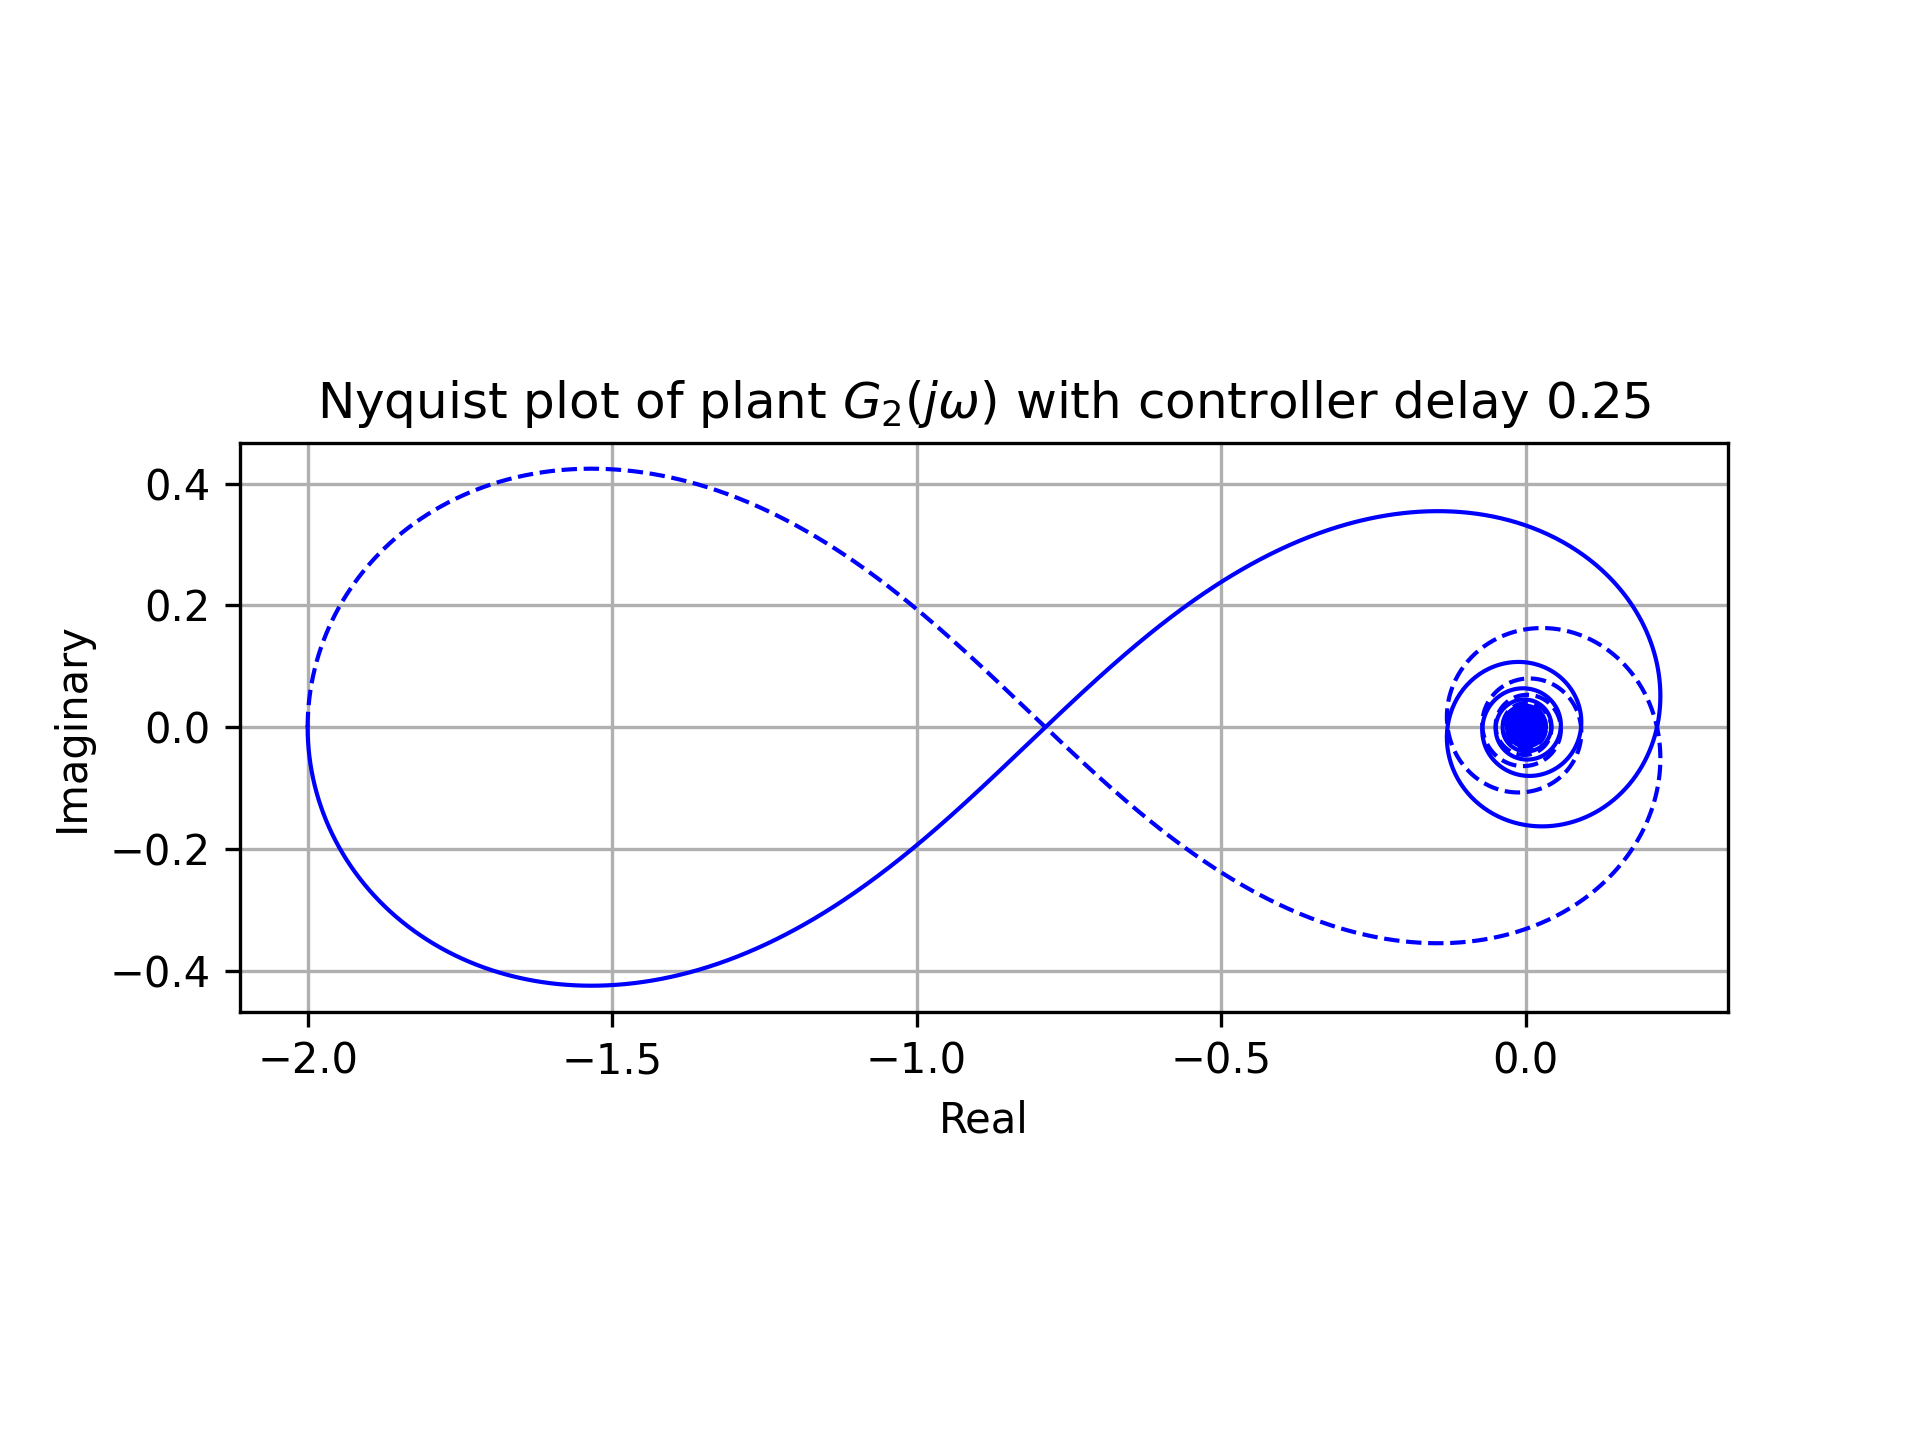
\includegraphics[width=0.8\textwidth]{figures/nyquist3.png}
    \caption{Nyquist plot of plant, $G_2(j\omega)$}
    \label{fig:nyquist3}
\end{figure}

\section{Autopilot}

\begin{equation}
    G_3(s) = \frac{6.3s^2 + 4.3s + 0.28}{s^5 + 11.2s^4 + 19.6s^3 + 16.2s^2 + 0.91s + 0.27}
\end{equation}

\subsection{A Proportional controller}

\begin{equation}
    u(t) = Ke(t)
\end{equation}

\begin{figure}[H]
    \centering
    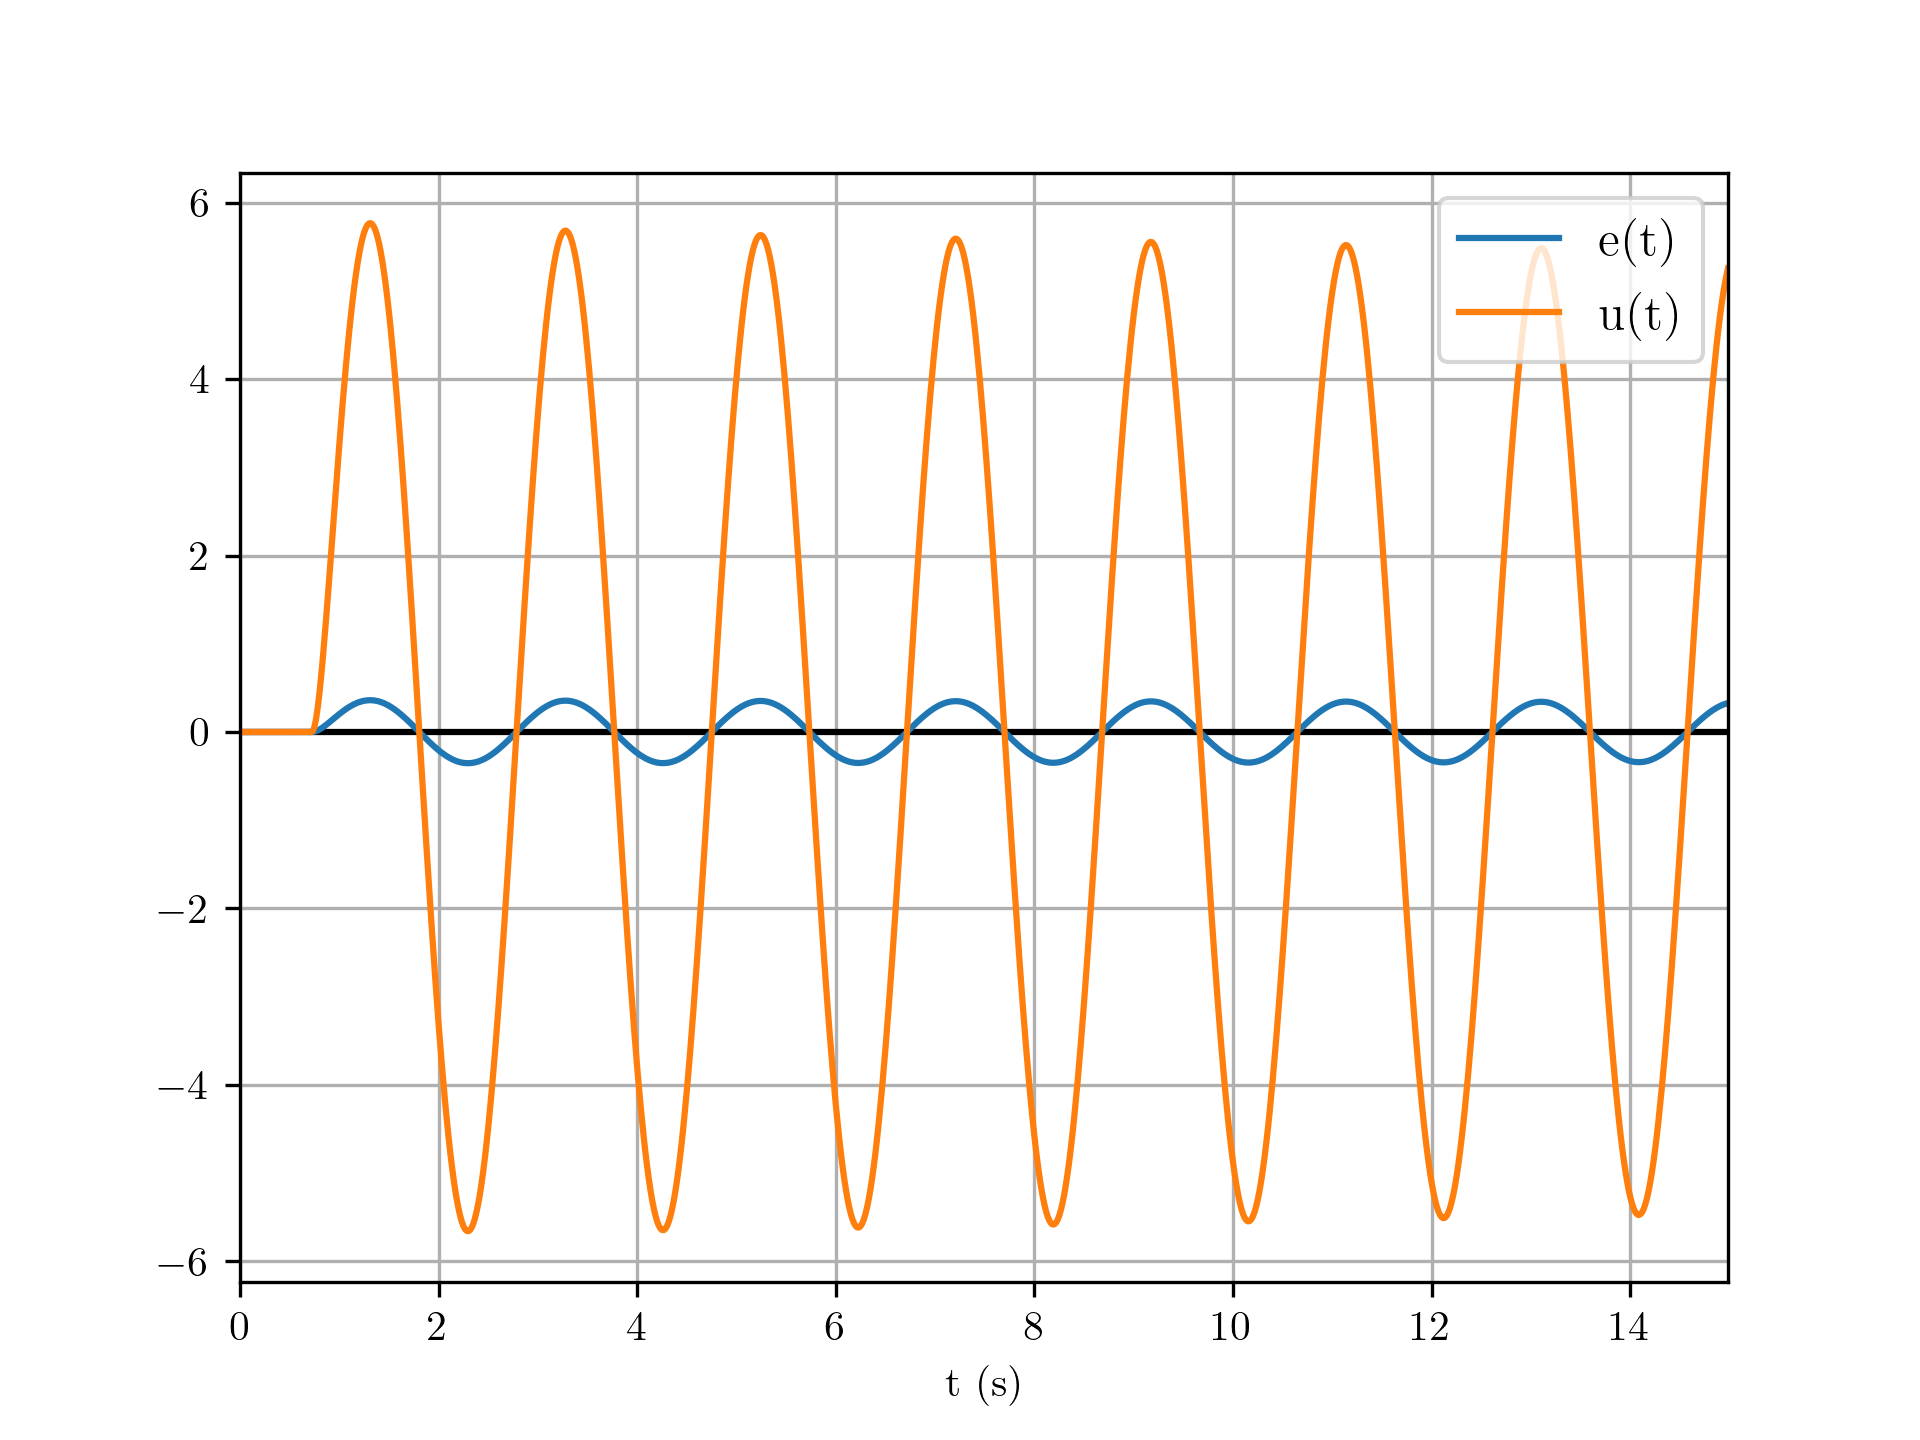
\includegraphics[width=0.8\textwidth]{figures/FIGURE_12.png}
    \caption{Figure 12}
    \label{fig:figure12}
\end{figure}

\subsection{A PID Controller}

\begin{equation}
    u(t) = K_p \left ( e(t) + \frac{1}{Ti}\int_{0}^{t}e(\tau)\mathrm{d}\tau + T_d\frac{\mathrm{d} e}{\mathrm{d} t} \right )
\end{equation}


Zieger Nichols tuned values
\begin{equation}
    K_p=0.6K_c, \;\;\;\; T_i=0.5T_c, \;\;\;\; T_d = 0.125T_c
\end{equation}

\begin{figure}[H]
    \centering
    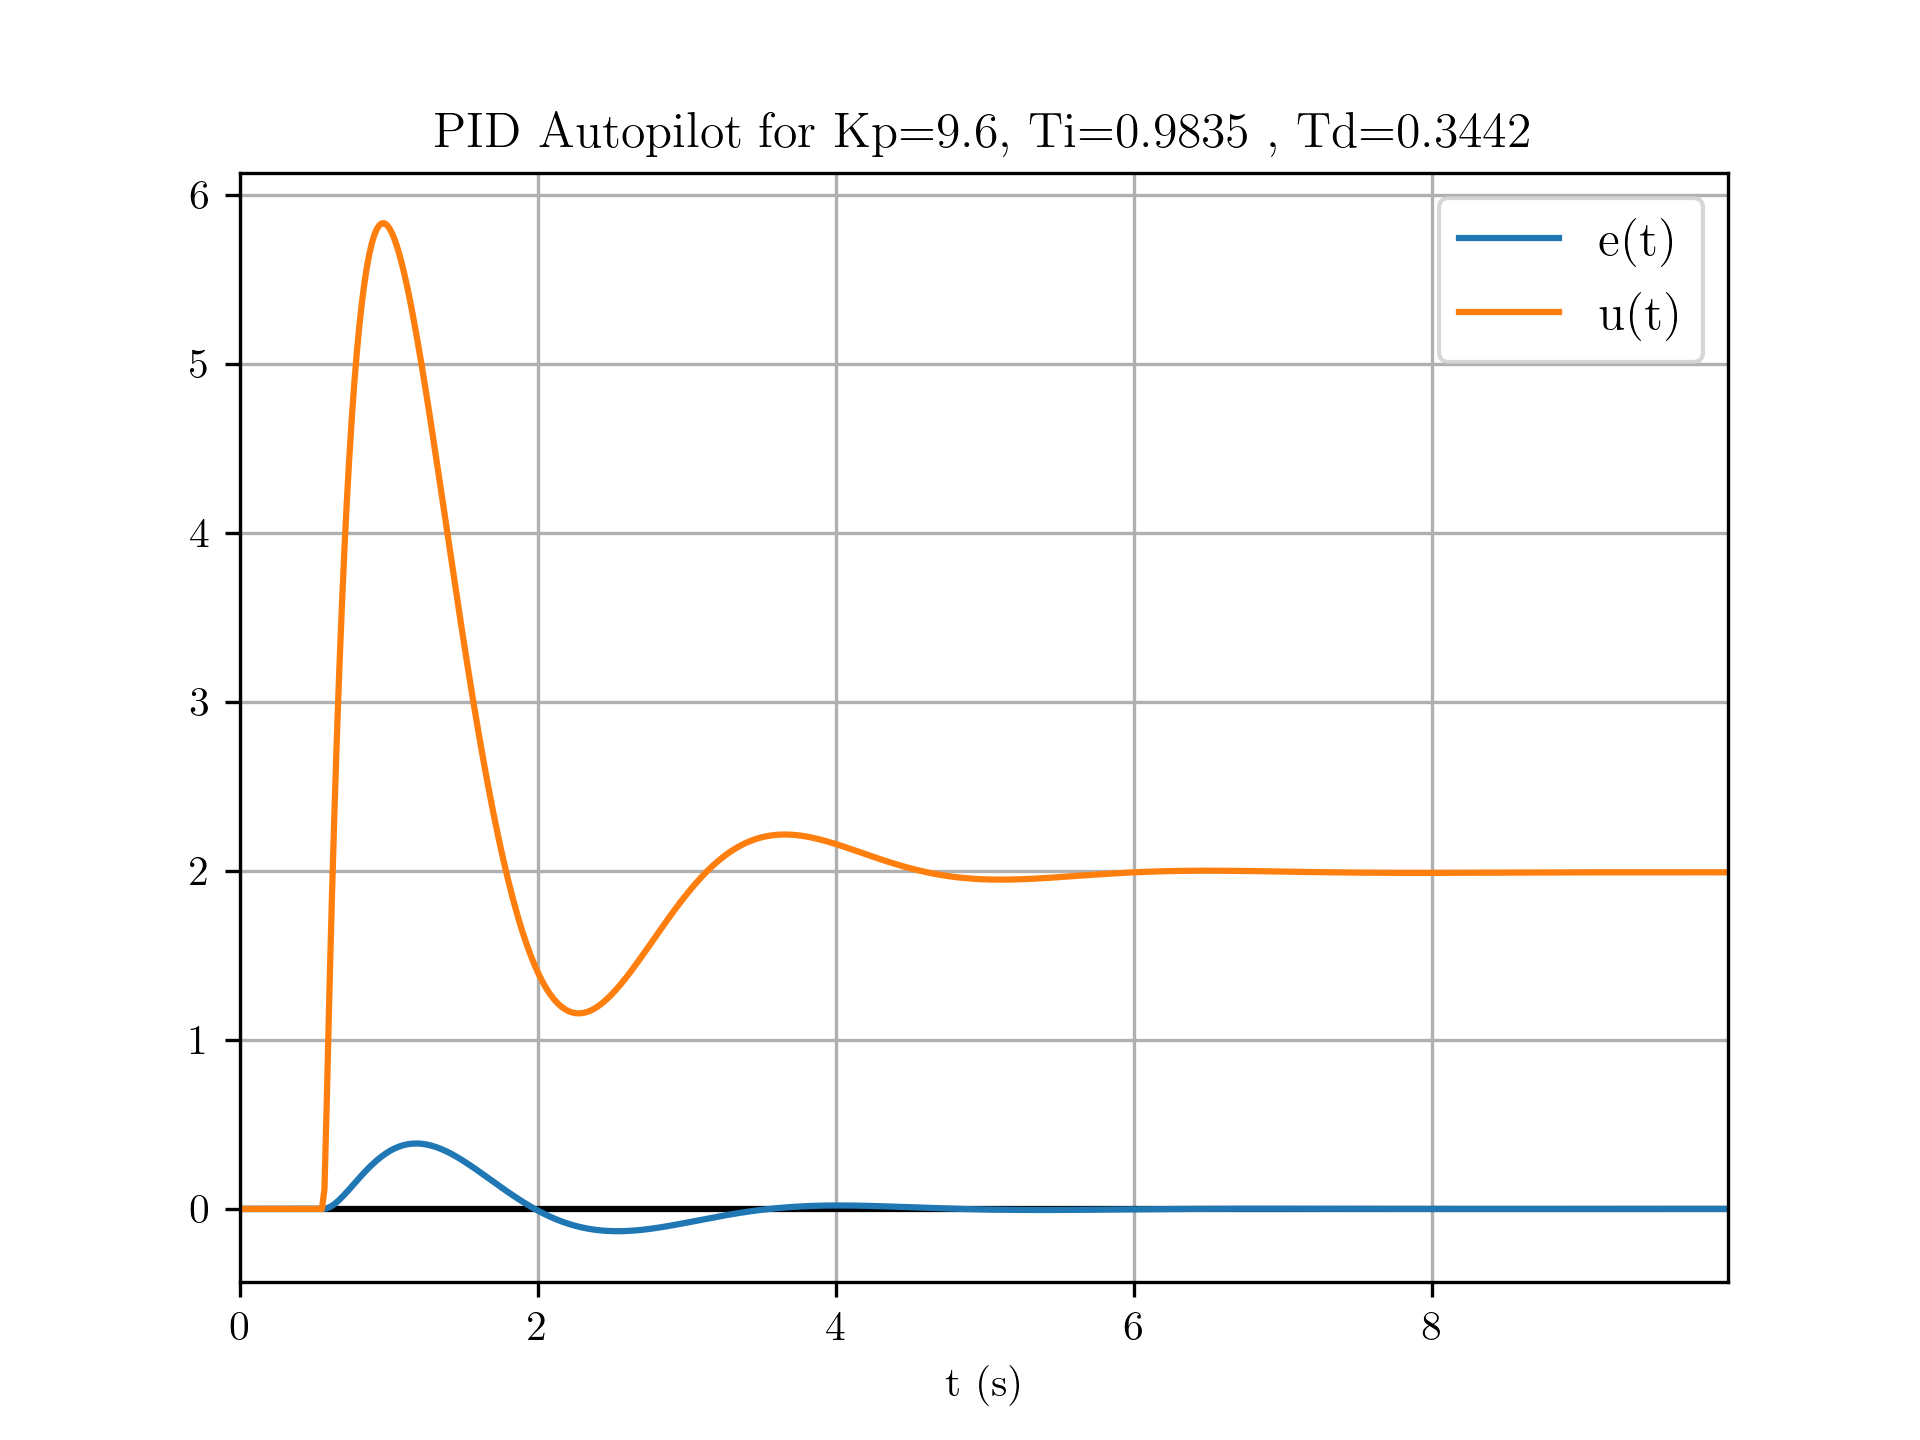
\includegraphics[width=0.8\textwidth]{figures/FIGURE_13.png}
    \caption{Figure 13}
    \label{fig:figure13}
\end{figure}


\subsection{Integrator wind up}

\begin{figure}[H]
    \centering
    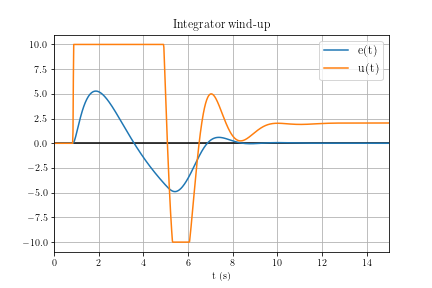
\includegraphics[width=0.8\textwidth]{figures/FIGURE_14.png}
    \caption{Figure 14}
    \label{fig:figure14}
\end{figure}

\begin{figure}[H]
    \centering
    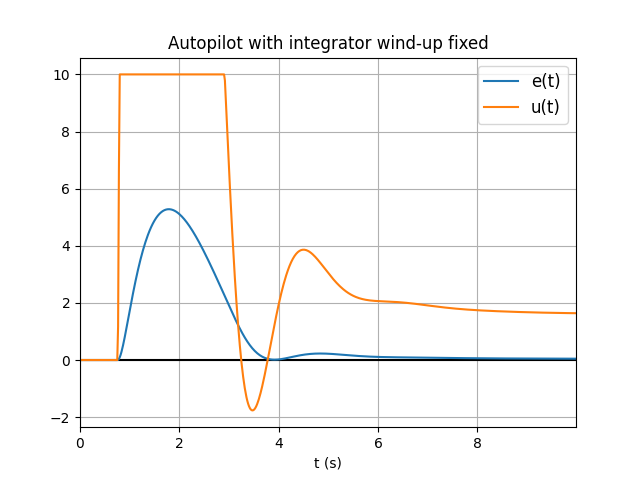
\includegraphics[width=0.8\textwidth]{figures/FIGURE_15.png}
    \caption{Figure 15}
    \label{fig:figure15}
\end{figure}

9. Explain your reasoning for this bound on $Q$


\subsection{Aims}

\begin{itemize}
\item To determine the 
\end{itemize}

\newpage

\section{Discussion}

%interpret results and comment on anomalies

\subsection{Improvements}

\section{Conclusion}

From the experiments performed it can be observed that blah blah blah

\end{document}
